\documentclass{article} % For LaTeX2e
\usepackage{iclr2025_conference,times}

% Optional math commands from https://github.com/goodfeli/dlbook_notation.
%%%%% NEW MATH DEFINITIONS %%%%%

\usepackage{amsmath,amsfonts,bm}

% Mark sections of captions for referring to divisions of figures
\newcommand{\figleft}{{\em (Left)}}
\newcommand{\figcenter}{{\em (Center)}}
\newcommand{\figright}{{\em (Right)}}
\newcommand{\figtop}{{\em (Top)}}
\newcommand{\figbottom}{{\em (Bottom)}}
\newcommand{\captiona}{{\em (a)}}
\newcommand{\captionb}{{\em (b)}}
\newcommand{\captionc}{{\em (c)}}
\newcommand{\captiond}{{\em (d)}}

% Highlight a newly defined term
\newcommand{\newterm}[1]{{\bf #1}}


% Figure reference, lower-case.
\def\figref#1{figure~\ref{#1}}
% Figure reference, capital. For start of sentence
\def\Figref#1{Figure~\ref{#1}}
\def\twofigref#1#2{figures \ref{#1} and \ref{#2}}
\def\quadfigref#1#2#3#4{figures \ref{#1}, \ref{#2}, \ref{#3} and \ref{#4}}
% Section reference, lower-case.
\def\secref#1{section~\ref{#1}}
% Section reference, capital.
\def\Secref#1{Section~\ref{#1}}
% Reference to two sections.
\def\twosecrefs#1#2{sections \ref{#1} and \ref{#2}}
% Reference to three sections.
\def\secrefs#1#2#3{sections \ref{#1}, \ref{#2} and \ref{#3}}
% Reference to an equation, lower-case.
\def\eqref#1{equation~\ref{#1}}
% Reference to an equation, upper case
\def\Eqref#1{Equation~\ref{#1}}
% A raw reference to an equation---avoid using if possible
\def\plaineqref#1{\ref{#1}}
% Reference to a chapter, lower-case.
\def\chapref#1{chapter~\ref{#1}}
% Reference to an equation, upper case.
\def\Chapref#1{Chapter~\ref{#1}}
% Reference to a range of chapters
\def\rangechapref#1#2{chapters\ref{#1}--\ref{#2}}
% Reference to an algorithm, lower-case.
\def\algref#1{algorithm~\ref{#1}}
% Reference to an algorithm, upper case.
\def\Algref#1{Algorithm~\ref{#1}}
\def\twoalgref#1#2{algorithms \ref{#1} and \ref{#2}}
\def\Twoalgref#1#2{Algorithms \ref{#1} and \ref{#2}}
% Reference to a part, lower case
\def\partref#1{part~\ref{#1}}
% Reference to a part, upper case
\def\Partref#1{Part~\ref{#1}}
\def\twopartref#1#2{parts \ref{#1} and \ref{#2}}

\def\ceil#1{\lceil #1 \rceil}
\def\floor#1{\lfloor #1 \rfloor}
\def\1{\bm{1}}
\newcommand{\train}{\mathcal{D}}
\newcommand{\valid}{\mathcal{D_{\mathrm{valid}}}}
\newcommand{\test}{\mathcal{D_{\mathrm{test}}}}

\def\eps{{\epsilon}}


% Random variables
\def\reta{{\textnormal{$\eta$}}}
\def\ra{{\textnormal{a}}}
\def\rb{{\textnormal{b}}}
\def\rc{{\textnormal{c}}}
\def\rd{{\textnormal{d}}}
\def\re{{\textnormal{e}}}
\def\rf{{\textnormal{f}}}
\def\rg{{\textnormal{g}}}
\def\rh{{\textnormal{h}}}
\def\ri{{\textnormal{i}}}
\def\rj{{\textnormal{j}}}
\def\rk{{\textnormal{k}}}
\def\rl{{\textnormal{l}}}
% rm is already a command, just don't name any random variables m
\def\rn{{\textnormal{n}}}
\def\ro{{\textnormal{o}}}
\def\rp{{\textnormal{p}}}
\def\rq{{\textnormal{q}}}
\def\rr{{\textnormal{r}}}
\def\rs{{\textnormal{s}}}
\def\rt{{\textnormal{t}}}
\def\ru{{\textnormal{u}}}
\def\rv{{\textnormal{v}}}
\def\rw{{\textnormal{w}}}
\def\rx{{\textnormal{x}}}
\def\ry{{\textnormal{y}}}
\def\rz{{\textnormal{z}}}

% Random vectors
\def\rvepsilon{{\mathbf{\epsilon}}}
\def\rvtheta{{\mathbf{\theta}}}
\def\rva{{\mathbf{a}}}
\def\rvb{{\mathbf{b}}}
\def\rvc{{\mathbf{c}}}
\def\rvd{{\mathbf{d}}}
\def\rve{{\mathbf{e}}}
\def\rvf{{\mathbf{f}}}
\def\rvg{{\mathbf{g}}}
\def\rvh{{\mathbf{h}}}
\def\rvu{{\mathbf{i}}}
\def\rvj{{\mathbf{j}}}
\def\rvk{{\mathbf{k}}}
\def\rvl{{\mathbf{l}}}
\def\rvm{{\mathbf{m}}}
\def\rvn{{\mathbf{n}}}
\def\rvo{{\mathbf{o}}}
\def\rvp{{\mathbf{p}}}
\def\rvq{{\mathbf{q}}}
\def\rvr{{\mathbf{r}}}
\def\rvs{{\mathbf{s}}}
\def\rvt{{\mathbf{t}}}
\def\rvu{{\mathbf{u}}}
\def\rvv{{\mathbf{v}}}
\def\rvw{{\mathbf{w}}}
\def\rvx{{\mathbf{x}}}
\def\rvy{{\mathbf{y}}}
\def\rvz{{\mathbf{z}}}

% Elements of random vectors
\def\erva{{\textnormal{a}}}
\def\ervb{{\textnormal{b}}}
\def\ervc{{\textnormal{c}}}
\def\ervd{{\textnormal{d}}}
\def\erve{{\textnormal{e}}}
\def\ervf{{\textnormal{f}}}
\def\ervg{{\textnormal{g}}}
\def\ervh{{\textnormal{h}}}
\def\ervi{{\textnormal{i}}}
\def\ervj{{\textnormal{j}}}
\def\ervk{{\textnormal{k}}}
\def\ervl{{\textnormal{l}}}
\def\ervm{{\textnormal{m}}}
\def\ervn{{\textnormal{n}}}
\def\ervo{{\textnormal{o}}}
\def\ervp{{\textnormal{p}}}
\def\ervq{{\textnormal{q}}}
\def\ervr{{\textnormal{r}}}
\def\ervs{{\textnormal{s}}}
\def\ervt{{\textnormal{t}}}
\def\ervu{{\textnormal{u}}}
\def\ervv{{\textnormal{v}}}
\def\ervw{{\textnormal{w}}}
\def\ervx{{\textnormal{x}}}
\def\ervy{{\textnormal{y}}}
\def\ervz{{\textnormal{z}}}

% Random matrices
\def\rmA{{\mathbf{A}}}
\def\rmB{{\mathbf{B}}}
\def\rmC{{\mathbf{C}}}
\def\rmD{{\mathbf{D}}}
\def\rmE{{\mathbf{E}}}
\def\rmF{{\mathbf{F}}}
\def\rmG{{\mathbf{G}}}
\def\rmH{{\mathbf{H}}}
\def\rmI{{\mathbf{I}}}
\def\rmJ{{\mathbf{J}}}
\def\rmK{{\mathbf{K}}}
\def\rmL{{\mathbf{L}}}
\def\rmM{{\mathbf{M}}}
\def\rmN{{\mathbf{N}}}
\def\rmO{{\mathbf{O}}}
\def\rmP{{\mathbf{P}}}
\def\rmQ{{\mathbf{Q}}}
\def\rmR{{\mathbf{R}}}
\def\rmS{{\mathbf{S}}}
\def\rmT{{\mathbf{T}}}
\def\rmU{{\mathbf{U}}}
\def\rmV{{\mathbf{V}}}
\def\rmW{{\mathbf{W}}}
\def\rmX{{\mathbf{X}}}
\def\rmY{{\mathbf{Y}}}
\def\rmZ{{\mathbf{Z}}}

% Elements of random matrices
\def\ermA{{\textnormal{A}}}
\def\ermB{{\textnormal{B}}}
\def\ermC{{\textnormal{C}}}
\def\ermD{{\textnormal{D}}}
\def\ermE{{\textnormal{E}}}
\def\ermF{{\textnormal{F}}}
\def\ermG{{\textnormal{G}}}
\def\ermH{{\textnormal{H}}}
\def\ermI{{\textnormal{I}}}
\def\ermJ{{\textnormal{J}}}
\def\ermK{{\textnormal{K}}}
\def\ermL{{\textnormal{L}}}
\def\ermM{{\textnormal{M}}}
\def\ermN{{\textnormal{N}}}
\def\ermO{{\textnormal{O}}}
\def\ermP{{\textnormal{P}}}
\def\ermQ{{\textnormal{Q}}}
\def\ermR{{\textnormal{R}}}
\def\ermS{{\textnormal{S}}}
\def\ermT{{\textnormal{T}}}
\def\ermU{{\textnormal{U}}}
\def\ermV{{\textnormal{V}}}
\def\ermW{{\textnormal{W}}}
\def\ermX{{\textnormal{X}}}
\def\ermY{{\textnormal{Y}}}
\def\ermZ{{\textnormal{Z}}}

% Vectors
\def\vzero{{\bm{0}}}
\def\vone{{\bm{1}}}
\def\vmu{{\bm{\mu}}}
\def\vtheta{{\bm{\theta}}}
\def\va{{\bm{a}}}
\def\vb{{\bm{b}}}
\def\vc{{\bm{c}}}
\def\vd{{\bm{d}}}
\def\ve{{\bm{e}}}
\def\vf{{\bm{f}}}
\def\vg{{\bm{g}}}
\def\vh{{\bm{h}}}
\def\vi{{\bm{i}}}
\def\vj{{\bm{j}}}
\def\vk{{\bm{k}}}
\def\vl{{\bm{l}}}
\def\vm{{\bm{m}}}
\def\vn{{\bm{n}}}
\def\vo{{\bm{o}}}
\def\vp{{\bm{p}}}
\def\vq{{\bm{q}}}
\def\vr{{\bm{r}}}
\def\vs{{\bm{s}}}
\def\vt{{\bm{t}}}
\def\vu{{\bm{u}}}
\def\vv{{\bm{v}}}
\def\vw{{\bm{w}}}
\def\vx{{\bm{x}}}
\def\vy{{\bm{y}}}
\def\vz{{\bm{z}}}

% Elements of vectors
\def\evalpha{{\alpha}}
\def\evbeta{{\beta}}
\def\evepsilon{{\epsilon}}
\def\evlambda{{\lambda}}
\def\evomega{{\omega}}
\def\evmu{{\mu}}
\def\evpsi{{\psi}}
\def\evsigma{{\sigma}}
\def\evtheta{{\theta}}
\def\eva{{a}}
\def\evb{{b}}
\def\evc{{c}}
\def\evd{{d}}
\def\eve{{e}}
\def\evf{{f}}
\def\evg{{g}}
\def\evh{{h}}
\def\evi{{i}}
\def\evj{{j}}
\def\evk{{k}}
\def\evl{{l}}
\def\evm{{m}}
\def\evn{{n}}
\def\evo{{o}}
\def\evp{{p}}
\def\evq{{q}}
\def\evr{{r}}
\def\evs{{s}}
\def\evt{{t}}
\def\evu{{u}}
\def\evv{{v}}
\def\evw{{w}}
\def\evx{{x}}
\def\evy{{y}}
\def\evz{{z}}

% Matrix
\def\mA{{\bm{A}}}
\def\mB{{\bm{B}}}
\def\mC{{\bm{C}}}
\def\mD{{\bm{D}}}
\def\mE{{\bm{E}}}
\def\mF{{\bm{F}}}
\def\mG{{\bm{G}}}
\def\mH{{\bm{H}}}
\def\mI{{\bm{I}}}
\def\mJ{{\bm{J}}}
\def\mK{{\bm{K}}}
\def\mL{{\bm{L}}}
\def\mM{{\bm{M}}}
\def\mN{{\bm{N}}}
\def\mO{{\bm{O}}}
\def\mP{{\bm{P}}}
\def\mQ{{\bm{Q}}}
\def\mR{{\bm{R}}}
\def\mS{{\bm{S}}}
\def\mT{{\bm{T}}}
\def\mU{{\bm{U}}}
\def\mV{{\bm{V}}}
\def\mW{{\bm{W}}}
\def\mX{{\bm{X}}}
\def\mY{{\bm{Y}}}
\def\mZ{{\bm{Z}}}
\def\mBeta{{\bm{\beta}}}
\def\mPhi{{\bm{\Phi}}}
\def\mLambda{{\bm{\Lambda}}}
\def\mSigma{{\bm{\Sigma}}}

% Tensor
\DeclareMathAlphabet{\mathsfit}{\encodingdefault}{\sfdefault}{m}{sl}
\SetMathAlphabet{\mathsfit}{bold}{\encodingdefault}{\sfdefault}{bx}{n}
\newcommand{\tens}[1]{\bm{\mathsfit{#1}}}
\def\tA{{\tens{A}}}
\def\tB{{\tens{B}}}
\def\tC{{\tens{C}}}
\def\tD{{\tens{D}}}
\def\tE{{\tens{E}}}
\def\tF{{\tens{F}}}
\def\tG{{\tens{G}}}
\def\tH{{\tens{H}}}
\def\tI{{\tens{I}}}
\def\tJ{{\tens{J}}}
\def\tK{{\tens{K}}}
\def\tL{{\tens{L}}}
\def\tM{{\tens{M}}}
\def\tN{{\tens{N}}}
\def\tO{{\tens{O}}}
\def\tP{{\tens{P}}}
\def\tQ{{\tens{Q}}}
\def\tR{{\tens{R}}}
\def\tS{{\tens{S}}}
\def\tT{{\tens{T}}}
\def\tU{{\tens{U}}}
\def\tV{{\tens{V}}}
\def\tW{{\tens{W}}}
\def\tX{{\tens{X}}}
\def\tY{{\tens{Y}}}
\def\tZ{{\tens{Z}}}


% Graph
\def\gA{{\mathcal{A}}}
\def\gB{{\mathcal{B}}}
\def\gC{{\mathcal{C}}}
\def\gD{{\mathcal{D}}}
\def\gE{{\mathcal{E}}}
\def\gF{{\mathcal{F}}}
\def\gG{{\mathcal{G}}}
\def\gH{{\mathcal{H}}}
\def\gI{{\mathcal{I}}}
\def\gJ{{\mathcal{J}}}
\def\gK{{\mathcal{K}}}
\def\gL{{\mathcal{L}}}
\def\gM{{\mathcal{M}}}
\def\gN{{\mathcal{N}}}
\def\gO{{\mathcal{O}}}
\def\gP{{\mathcal{P}}}
\def\gQ{{\mathcal{Q}}}
\def\gR{{\mathcal{R}}}
\def\gS{{\mathcal{S}}}
\def\gT{{\mathcal{T}}}
\def\gU{{\mathcal{U}}}
\def\gV{{\mathcal{V}}}
\def\gW{{\mathcal{W}}}
\def\gX{{\mathcal{X}}}
\def\gY{{\mathcal{Y}}}
\def\gZ{{\mathcal{Z}}}

% Sets
\def\sA{{\mathbb{A}}}
\def\sB{{\mathbb{B}}}
\def\sC{{\mathbb{C}}}
\def\sD{{\mathbb{D}}}
% Don't use a set called E, because this would be the same as our symbol
% for expectation.
\def\sF{{\mathbb{F}}}
\def\sG{{\mathbb{G}}}
\def\sH{{\mathbb{H}}}
\def\sI{{\mathbb{I}}}
\def\sJ{{\mathbb{J}}}
\def\sK{{\mathbb{K}}}
\def\sL{{\mathbb{L}}}
\def\sM{{\mathbb{M}}}
\def\sN{{\mathbb{N}}}
\def\sO{{\mathbb{O}}}
\def\sP{{\mathbb{P}}}
\def\sQ{{\mathbb{Q}}}
\def\sR{{\mathbb{R}}}
\def\sS{{\mathbb{S}}}
\def\sT{{\mathbb{T}}}
\def\sU{{\mathbb{U}}}
\def\sV{{\mathbb{V}}}
\def\sW{{\mathbb{W}}}
\def\sX{{\mathbb{X}}}
\def\sY{{\mathbb{Y}}}
\def\sZ{{\mathbb{Z}}}

% Entries of a matrix
\def\emLambda{{\Lambda}}
\def\emA{{A}}
\def\emB{{B}}
\def\emC{{C}}
\def\emD{{D}}
\def\emE{{E}}
\def\emF{{F}}
\def\emG{{G}}
\def\emH{{H}}
\def\emI{{I}}
\def\emJ{{J}}
\def\emK{{K}}
\def\emL{{L}}
\def\emM{{M}}
\def\emN{{N}}
\def\emO{{O}}
\def\emP{{P}}
\def\emQ{{Q}}
\def\emR{{R}}
\def\emS{{S}}
\def\emT{{T}}
\def\emU{{U}}
\def\emV{{V}}
\def\emW{{W}}
\def\emX{{X}}
\def\emY{{Y}}
\def\emZ{{Z}}
\def\emSigma{{\Sigma}}

% entries of a tensor
% Same font as tensor, without \bm wrapper
\newcommand{\etens}[1]{\mathsfit{#1}}
\def\etLambda{{\etens{\Lambda}}}
\def\etA{{\etens{A}}}
\def\etB{{\etens{B}}}
\def\etC{{\etens{C}}}
\def\etD{{\etens{D}}}
\def\etE{{\etens{E}}}
\def\etF{{\etens{F}}}
\def\etG{{\etens{G}}}
\def\etH{{\etens{H}}}
\def\etI{{\etens{I}}}
\def\etJ{{\etens{J}}}
\def\etK{{\etens{K}}}
\def\etL{{\etens{L}}}
\def\etM{{\etens{M}}}
\def\etN{{\etens{N}}}
\def\etO{{\etens{O}}}
\def\etP{{\etens{P}}}
\def\etQ{{\etens{Q}}}
\def\etR{{\etens{R}}}
\def\etS{{\etens{S}}}
\def\etT{{\etens{T}}}
\def\etU{{\etens{U}}}
\def\etV{{\etens{V}}}
\def\etW{{\etens{W}}}
\def\etX{{\etens{X}}}
\def\etY{{\etens{Y}}}
\def\etZ{{\etens{Z}}}

% The true underlying data generating distribution
\newcommand{\pdata}{p_{\rm{data}}}
% The empirical distribution defined by the training set
\newcommand{\ptrain}{\hat{p}_{\rm{data}}}
\newcommand{\Ptrain}{\hat{P}_{\rm{data}}}
% The model distribution
\newcommand{\pmodel}{p_{\rm{model}}}
\newcommand{\Pmodel}{P_{\rm{model}}}
\newcommand{\ptildemodel}{\tilde{p}_{\rm{model}}}
% Stochastic autoencoder distributions
\newcommand{\pencode}{p_{\rm{encoder}}}
\newcommand{\pdecode}{p_{\rm{decoder}}}
\newcommand{\precons}{p_{\rm{reconstruct}}}

\newcommand{\laplace}{\mathrm{Laplace}} % Laplace distribution

\newcommand{\E}{\mathbb{E}}
\newcommand{\Ls}{\mathcal{L}}
\newcommand{\R}{\mathbb{R}}
\newcommand{\emp}{\tilde{p}}
\newcommand{\lr}{\alpha}
\newcommand{\reg}{\lambda}
\newcommand{\rect}{\mathrm{rectifier}}
\newcommand{\softmax}{\mathrm{softmax}}
\newcommand{\sigmoid}{\sigma}
\newcommand{\softplus}{\zeta}
\newcommand{\KL}{D_{\mathrm{KL}}}
\newcommand{\Var}{\mathrm{Var}}
\newcommand{\standarderror}{\mathrm{SE}}
\newcommand{\Cov}{\mathrm{Cov}}
% Wolfram Mathworld says $L^2$ is for function spaces and $\ell^2$ is for vectors
% But then they seem to use $L^2$ for vectors throughout the site, and so does
% wikipedia.
\newcommand{\normlzero}{L^0}
\newcommand{\normlone}{L^1}
\newcommand{\normltwo}{L^2}
\newcommand{\normlp}{L^p}
\newcommand{\normmax}{L^\infty}

\newcommand{\parents}{Pa} % See usage in notation.tex. Chosen to match Daphne's book.

\DeclareMathOperator*{\argmax}{arg\,max}
\DeclareMathOperator*{\argmin}{arg\,min}

\DeclareMathOperator{\sign}{sign}
\DeclareMathOperator{\Tr}{Tr}
\let\ab\allowbreak


% \usepackage{hyperref}
\usepackage{url}



\usepackage[utf8]{inputenc}         %
\usepackage[T1]{fontenc}            %
\usepackage{url}                    %
\usepackage{booktabs}               %
\usepackage{amsfonts}               %
\usepackage{nicefrac}               %
\usepackage{microtype}              %
\usepackage{xcolor}                 %
\usepackage{algorithm}
\usepackage{algorithmic}
\usepackage{graphicx}
\usepackage{subcaption}
\usepackage[flushleft]{threeparttable}
\usepackage{float}
\usepackage{multirow}
\usepackage{xspace}
\usepackage{natbib}
\usepackage{enumitem}
\usepackage[font=small]{caption}
\usepackage{autobreak}
\usepackage{sidecap}
\usepackage{wrapfig}
\usepackage{bbding}
\usepackage[toc, page, header]{appendix}
\usepackage{tikz}
\usepackage{xcolor}
\usepackage{pifont}
\usepackage{mdframed}
\usepackage{colortbl}
\usepackage{mathrsfs}
\usepackage[textwidth=3.4cm,textsize=tiny]{todonotes}
% \usepackage{booktabs}
\usepackage{longtable}

\usepackage[colorlinks=true, linkcolor=blue, citecolor=blue, urlcolor=blue]{hyperref}


\newcommand{\kang}[1]{\todo[color=yellow!20,size=\footnotesize,caption={}]{K: #1}{}}
\newcommand{\ikang}[1]{\todo[inline,color=yellow!20,size=\footnotesize,caption={}]{K: #1}{}}

\newcommand{\tao}[1]{\todo[color=blue!20,size=\footnotesize,caption={}]{T: #1}{}}
\newcommand{\itao}[1]{\todo[inline,color=blue!20,size=\footnotesize,caption={}]{T: #1}{}}

\newcommand{\bu}[1]{\todo[color=green!20,size=\footnotesize,caption={}]{S: #1}{}}
\newcommand{\ibu}[1]{\todo[inline,color=green!20,size=\footnotesize,caption={}]{S: #1}{}}

\newcommand{\greentext}[1]{\textcolor{green!50!black}{#1}}
\newcommand{\orangetext}[1]{\textcolor{orange!75!black}{#1}}
\newcommand{\purpletext}[1]{\textcolor{purple!75!black}{#1}}
\newcommand{\bluetext}[1]{\textcolor{blue!50!black}{#1}}
\newcommand{\redtext}[1]{\textcolor{red!75!black}{#1}}

\title{Clustering the automotive}

% Authors must not appear in the submitted version. They should be hidden
% as long as the \iclrfinalcopy macro remains commented out below.
% Non-anonymous submissions will be rejected without review.

% \author{Antiquus S.~Hippocampus, Natalia Cerebro \& Amelie P. Amygdale \thanks{ Use footnote for providing further information
% about author (webpage, alternative address)---\emph{not} for acknowledging
% funding agencies.  Funding acknowledgements go at the end of the paper.} \\
% Department of Computer Science\\
% Cranberry-Lemon University\\
% Pittsburgh, PA 15213, USA \\
% \texttt{\{hippo,brain,jen\}@cs.cranberry-lemon.edu} \\
% \And
% Ji Q. Ren \& Yevgeny LeNet \\
% Department of Computational Neuroscience \\
% University of the Witwatersrand \\
% Joburg, South Africa \\
% \texttt{\{robot,net\}@wits.ac.za} \\
% \AND
% Coauthor \\
% Affiliation \\
% Address \\
% \texttt{email}
% }

\author{Runkang Yang\thanks{Project Leader.}, Panxin Tao\thanks{Equal contribution.}, Zhuoyang Bu\footnotemark[2]\\
\texttt{\{yangrk2022,taopx2022,buzy2022\}@shanghaitech.edu.cn}}

% The \author macro works with any number of authors. There are two commands
% used to separate the names and addresses of multiple authors: \And and \AND.
%
% Using \And between authors leaves it to \LaTeX{} to determine where to break
% the lines. Using \AND forces a linebreak at that point. So, if \LaTeX{}
% puts 3 of 4 authors names on the first line, and the last on the second
% line, try using \AND instead of \And before the third author name.

\newcommand{\fix}{\marginpar{FIX}}
\newcommand{\new}{\marginpar{NEW}}

\iclrfinalcopy % Uncomment for camera-ready version, but NOT for submission.
\begin{document}


\maketitle


\begin{abstract}
   Clustering analysis plays a pivotal role in identifying patterns within complex datasets and can be particularly valuable for competitor analysis in automotive industry, 
   This study addresses the challenge of identifying competing vehicles for Volkswagen.
   We first conduct Principal Component Analysis (PCA) and AutoEncoder for dimensionality reduction, followed by K-means and hierarchical clustering for product segmentation. 
   Through qualitative analysis and quantitative comparison, we empirically find that \textit{the combination of AE for feature extraction and HC for clustering appears to be the most effective approach}. It not only achieves the \purpletext{best clustering evaluation metrics} but also results in a logical grouping of vehicles that reflects market segmentation.
   % We emphasizes the advantages of AutoEncoder-based dimensionality reduction, particularly in its ability to handle high-dimensional data and preserve critical feature relationships than traditional methods. 
   This research not only advances the application of clustering methods in automotive sales industry but also illustrates the potential of deep learning techniques used in high-dimensional data spaces.
\end{abstract}


\begin{figure}[!ht]
   \centering
   \begin{subfigure}{.49\textwidth}
       \centering
       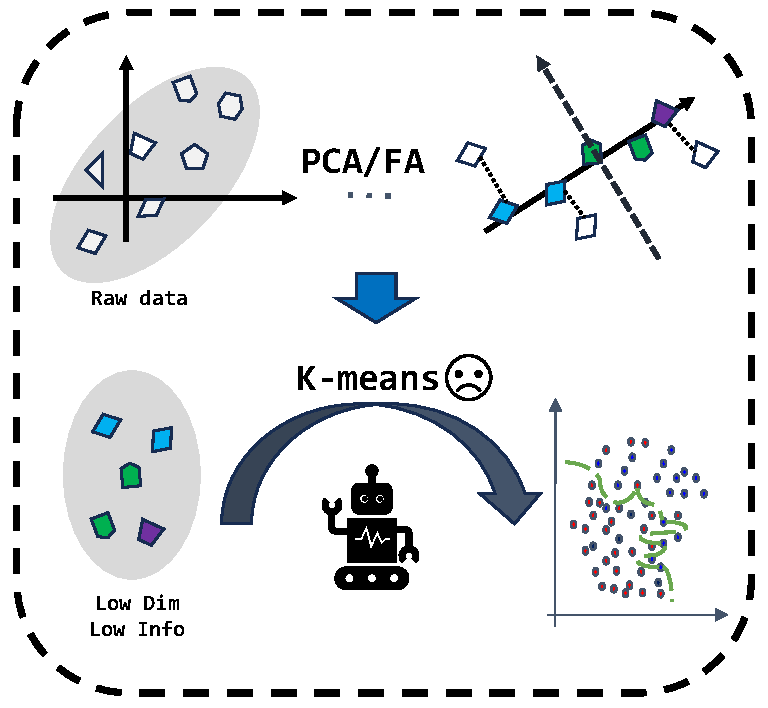
\includegraphics[width=1.0\linewidth]{./figures/PCA.pdf}
       \vspace{-5pt}
       \label{fig:sketch1}
   \end{subfigure}
   \hfill
   \begin{subfigure}{.49\textwidth}
       \centering
       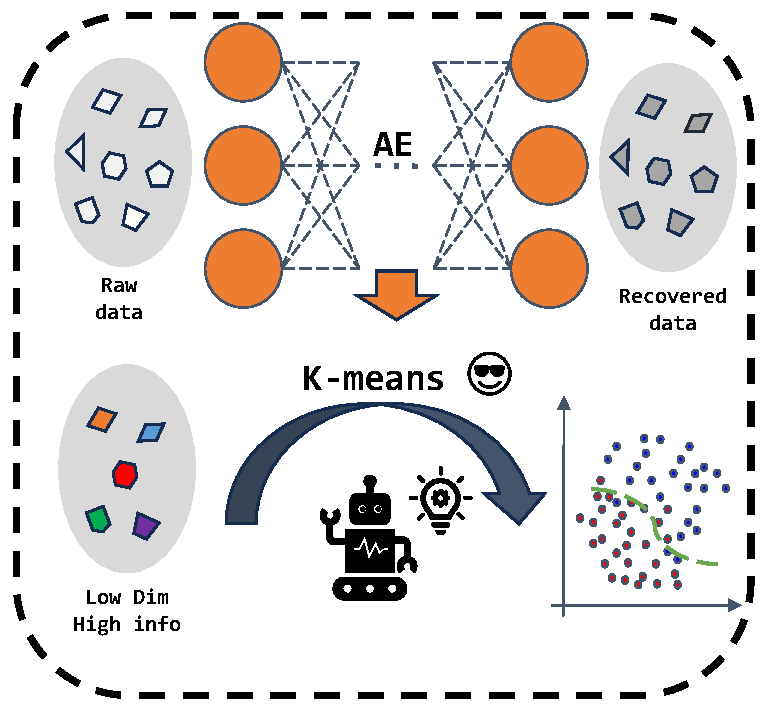
\includegraphics[width=1.0\linewidth]{./figures/AE.pdf}
       \vspace{-5pt}
       \label{fig:sketch2}
   \end{subfigure}
   \caption{\textbf{Traditional PCA-based dimensionality reduction (left) and neural network-based autoencoder dimensionality reduction (right).} Traditional PCA/FA relies on linear transformations, which inherently possess limitations in capturing nonlinear patterns in data. In contrast, neural network-based autoencoders leverage nonlinearity and hierarchical feature extraction, enabling them to handle complex data distributions effectively, thus contributes to downstream clustering tasks.}
   \label{fig:sketch}
   \vspace{-12pt}
\end{figure}


\section{Introduction}

Clustering analysis is a widely used technique for identifying patterns in large and complex datasets, making it particularly useful in fields such as market segmentation, product grouping, and competitor analysis.
In the automotive industry, clustering can be an invaluable tool for identifying groups of similar vehicles, which can inform product positioning, pricing strategies, and competitive analysis.

To perform effective clustering, it is crucial to reduce the dimensionality of the data while preserving its key structure.
Traditional methods, such as Principal Component Analysis (PCA), have long been used for this purpose by transforming the original feature space into a set of uncorrelated components that capture the most significant variance in the data~\citep{pearson1901pca,hotelling1933pca}.
However, PCA often struggles to capture non-linear relationships, which are prevalent in real-world datasets like automotive data in this problem.

To address these limitations, more recent methods have leveraged deep learning techniques, particularly AutoEncoders (AE), for dimensionality reduction.
AutoEncoders are neural network-based models that learn a compressed representation of the input data in a lower-dimensional space, capable of preserving complex, non-linear patterns~\citep{hinton2006autoencoder,goodfellow2016deep}.
By reducing the dimensionality of the data using AutoEncoders, we can extract more meaningful representations that can improve the performance of clustering algorithms.

After dimensionality reduction, clustering algorithms such as K-means~\citep{macqueen1967kmeans,jain2010kmeans} and hierarchical clustering~\citep{lance1967hierarchical,murtagh2012hierarchical} are commonly used to group vehicles based on their feature similarities.
K-means is a well-known clustering algorithm that works efficiently on large datasets and produces a predefined number of clusters based on the Euclidean distance between points.
However, K-means requires the number of clusters to be specified in advance and may struggle to detect clusters with non-spherical shapes. Hierarchical clustering, on the other hand, builds a tree of clusters and provides a more flexible approach to identifying relationships between data points.
After that, we quantitatively evaluate the clustering quality through internal metrics like the Silhouette Score(SC)~\citep{rousseeuw1987silhouettes}, Calinski-Harabasz Index(CH)~\citep{calinski1974dendrite}, Davies-Bouldin Index(DB)~\citep{davies1979cluster} and Dunn Index(DI)~\citep{dunn1974well}.

This paper aims to investigate the effectiveness of combining AutoEncoder-based dimensionality reduction with clustering methods for automotive competitor analysis.
Specifically, We detailed our methodology in~\autoref{sec:methodology}, mainly through comparing \orangetext{PCA} and \orangetext{AutoEncoder} for dimensionality reduction, followed by clustering with \orangetext{K-means} and \orangetext{hierarchical} methods.
And then present the numerical result in~\autoref{sec:numerical}, the conclusion in~\autoref{sec:conclusion}.

\section{Methodology}
\label{sec:methodology}

This section details the methodology employed for the analysis of the automotive dataset.
The approach includes data preprocessing, feature selection, and training of clustering models using two dimensionality reduction techniques: Principal Component Analysis (PCA) and AutoEncoders (AE).
Two clustering algorithms, K-means and hierarchical clustering, are then applied to identify competitor vehicles for Volkswagen, as shown in Figure~\ref{fig:sketch}, \ref{fig:pipeline}.

\subsection{Feature Engineering}


The first step involves preprocessing the dataset to ensure that it is ready for dimensionality reduction and clustering. This includes handling missing values, detecting and treating outliers, normalizing numerical data, and converting categorical variables into a format suitable for machine learning models.

The dataset has no missing value and except for the Car\_ID attribute which is only an index, we will divide the remaining attributes into two kind: categorical attributes and numerical attributes and handle them respectively.

\subsubsection{Data Cleaning}
This step involves correcting any errors present in the dataset, such as incorrect entries in categorical fields (e.g., misspelled car names or incorrect labels).
These issues were manually inspected and corrected by cross-referencing with external sources.
And in this problem, there is a typo in line 184 where \textit{vokswagen} refers to \textit{volkswagen}, and \textit{vw} is short for \textit{volkswagen}, we have manually identified and corrected them.

\subsubsection{One-hot Encoding of Categorical Variables}

In this section, we will handle the $10$ categorical attributes to fit them into the subsequent models.

First of all, we notice that the attributes doornumber and cylindernumber are expressed as number. We argue that the cylindernumber attribute has numerical significance and can be treated as a numerical attribute. On the other hand, the value of doornumber barely matters the choice of competitors, which should be treated as a categorical attribute.

We also notice that the CarName attribute has 147 different categories which is quite large and contains little useful information. Therefore, it will be extracted and handled as categorical attribute CarBrand subsequently. We observed misspelled or abbreviated categories in CarName, which should be corrected when extracting the CarBrand attribute.

After the data cleaning, one-hot encoding is applied to all the categorical attributes. We use one-hot encoding instead of label encoding because all the attributes have no ordinal relation.
% Categorical variables, such as \textit{fueltype} or \textit{carbody}, were transformed into a one-hot encoded representation. 
For a categorical variable \( C \) with \( N \) possible categories, each category was encoded as a binary vector.
For instance, if \( C = \{ \text{convertible}, \text{hatchback}, \text{sedan} \} \), the one-hot encoding would convert these categories into the following binary vectors:
$$
\text{convertible} = [1, 0, 0], \quad \text{hatchback} = [0, 1, 0], \quad \text{sedan} = [0, 0, 1]
$$

\subsubsection{Outlier Detection and Handling}
The remaining 15 numerical attributes and the cylindernumber attribute mentioned before are treated as numerical features.
Outliers in numerical features can significantly distort the analysis and modeling results. To detect and handle outliers, we utilized the z-score method, as shown in~\autoref{fig:Boxplot}. For a given numerical feature \( x_i \), the z-score is defined as:
$
z_i = \frac{x_i - \mu}{\sigma}
$
where \( \mu \) is the mean and \( \sigma \) is the standard deviation of the feature. Any data point with a z-score greater than 3 or less than -3 was considered an outlier and replaced by the median value of the corresponding feature \( \tilde{x} \):
$
x_i \leftarrow \tilde{x}
$

 \begin{figure}[t]
    \centering
    % \includegraphics[width=1.0\linewidth]{resources/figures/strategy.pdf}
    \begin{subfigure}{.49\textwidth}  % Adjust width to fit within the line
        \centering
        % \framebox[\linewidth][c]{\phantom{\rule{0pt}{0.918\linewidth}}}
        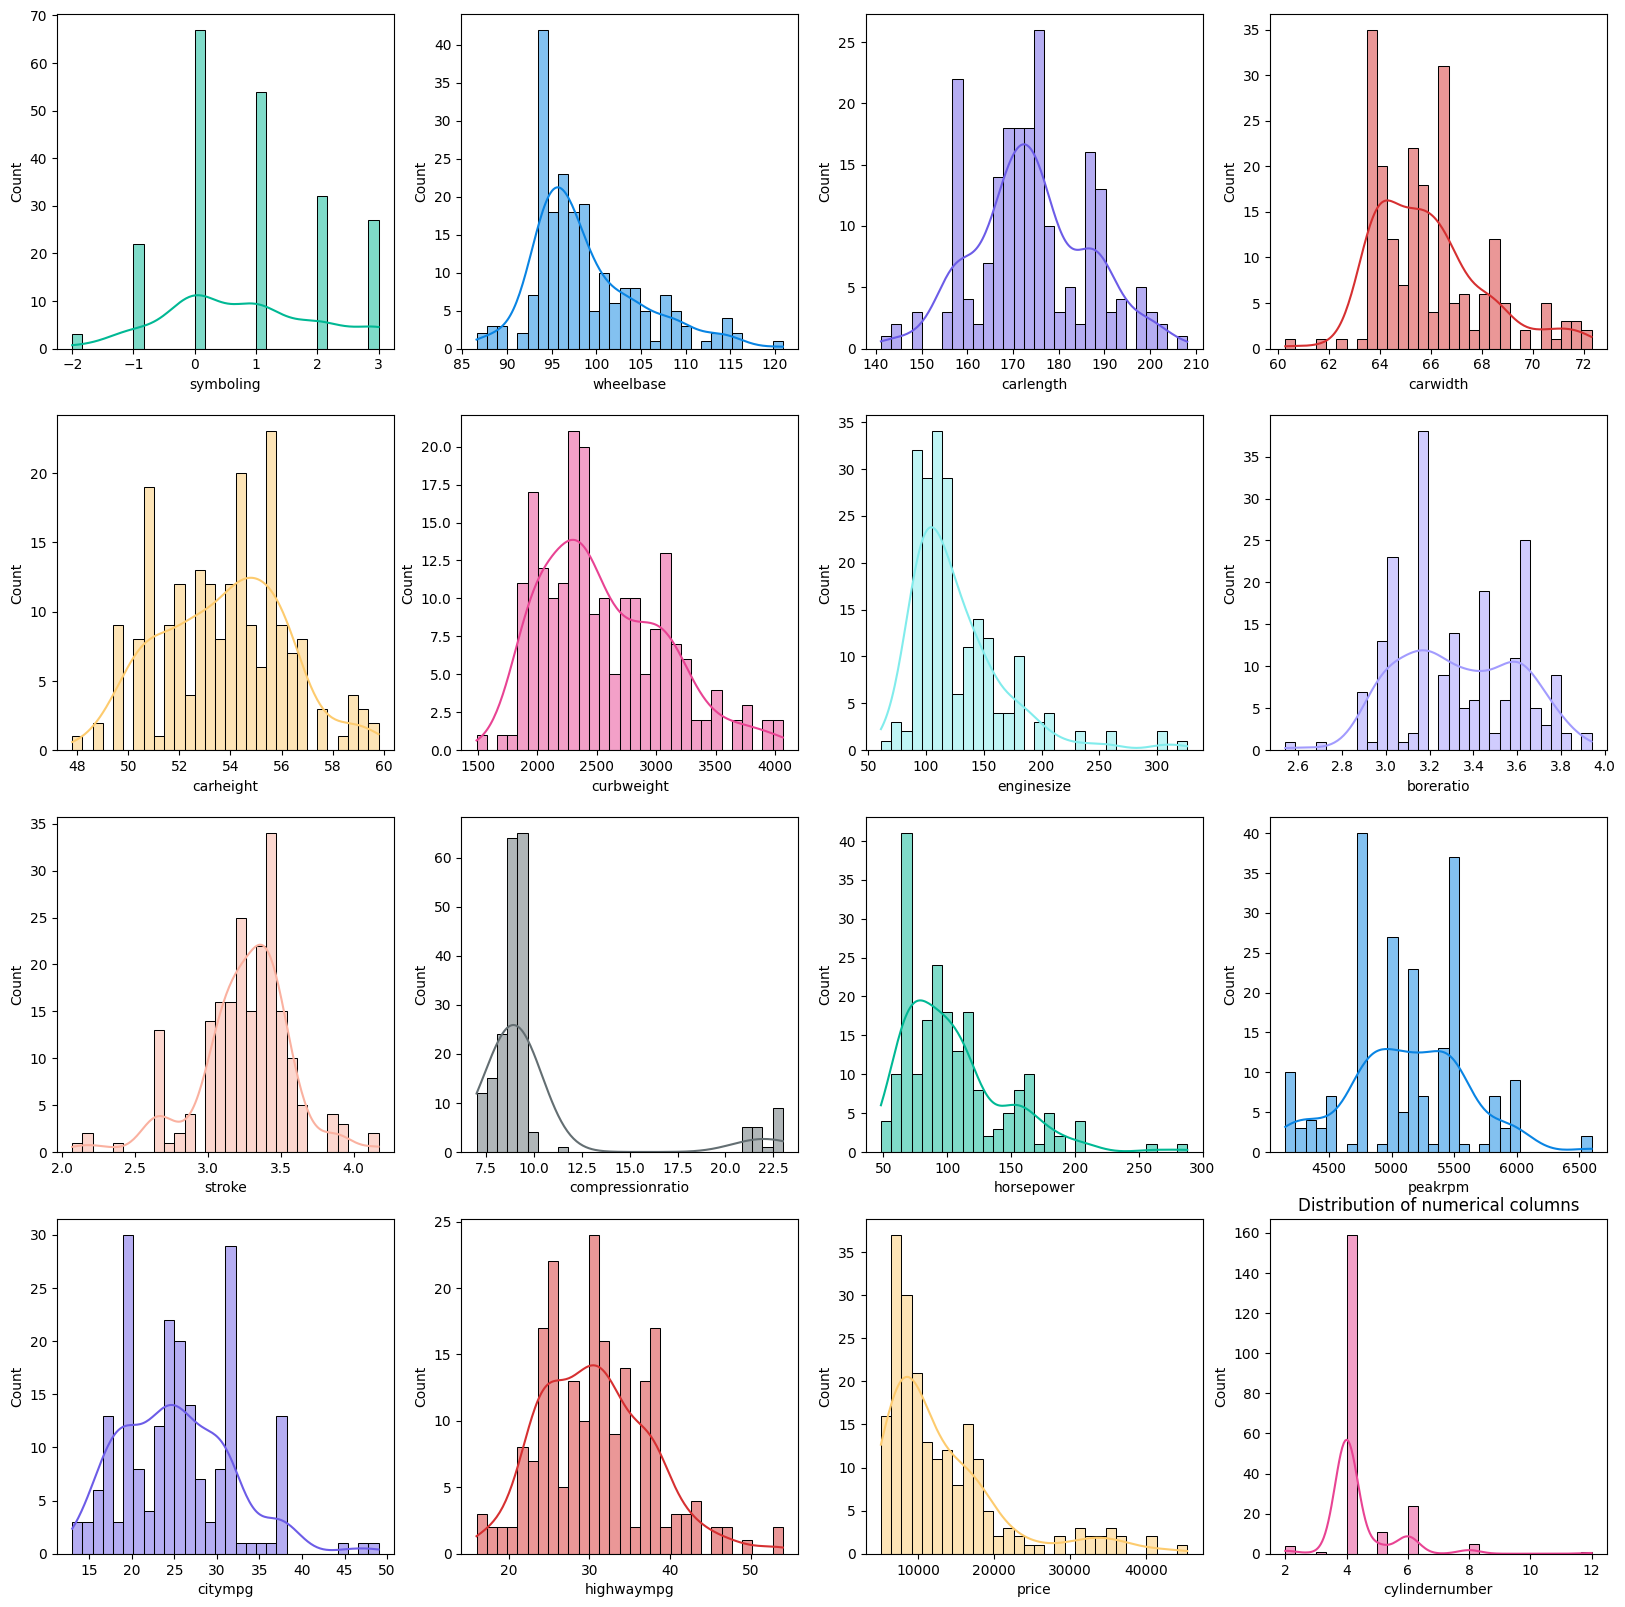
\includegraphics[width=1.0\linewidth]{./figures/data1.png}
        % \captionsetup{labelformat=empty,skip=-8pt}
        % \caption{Comparison \SA and \SB.}
        \label{fig:distribution}
        \vspace{-5pt}
    \end{subfigure}
    \hfill % Ensures that the subfigures are evenly spaced or fill the space
    \begin{subfigure}{.49\textwidth}
        \centering
        % \framebox[\linewidth][c]{\phantom{\rule{0pt}{0.918\linewidth}}}
        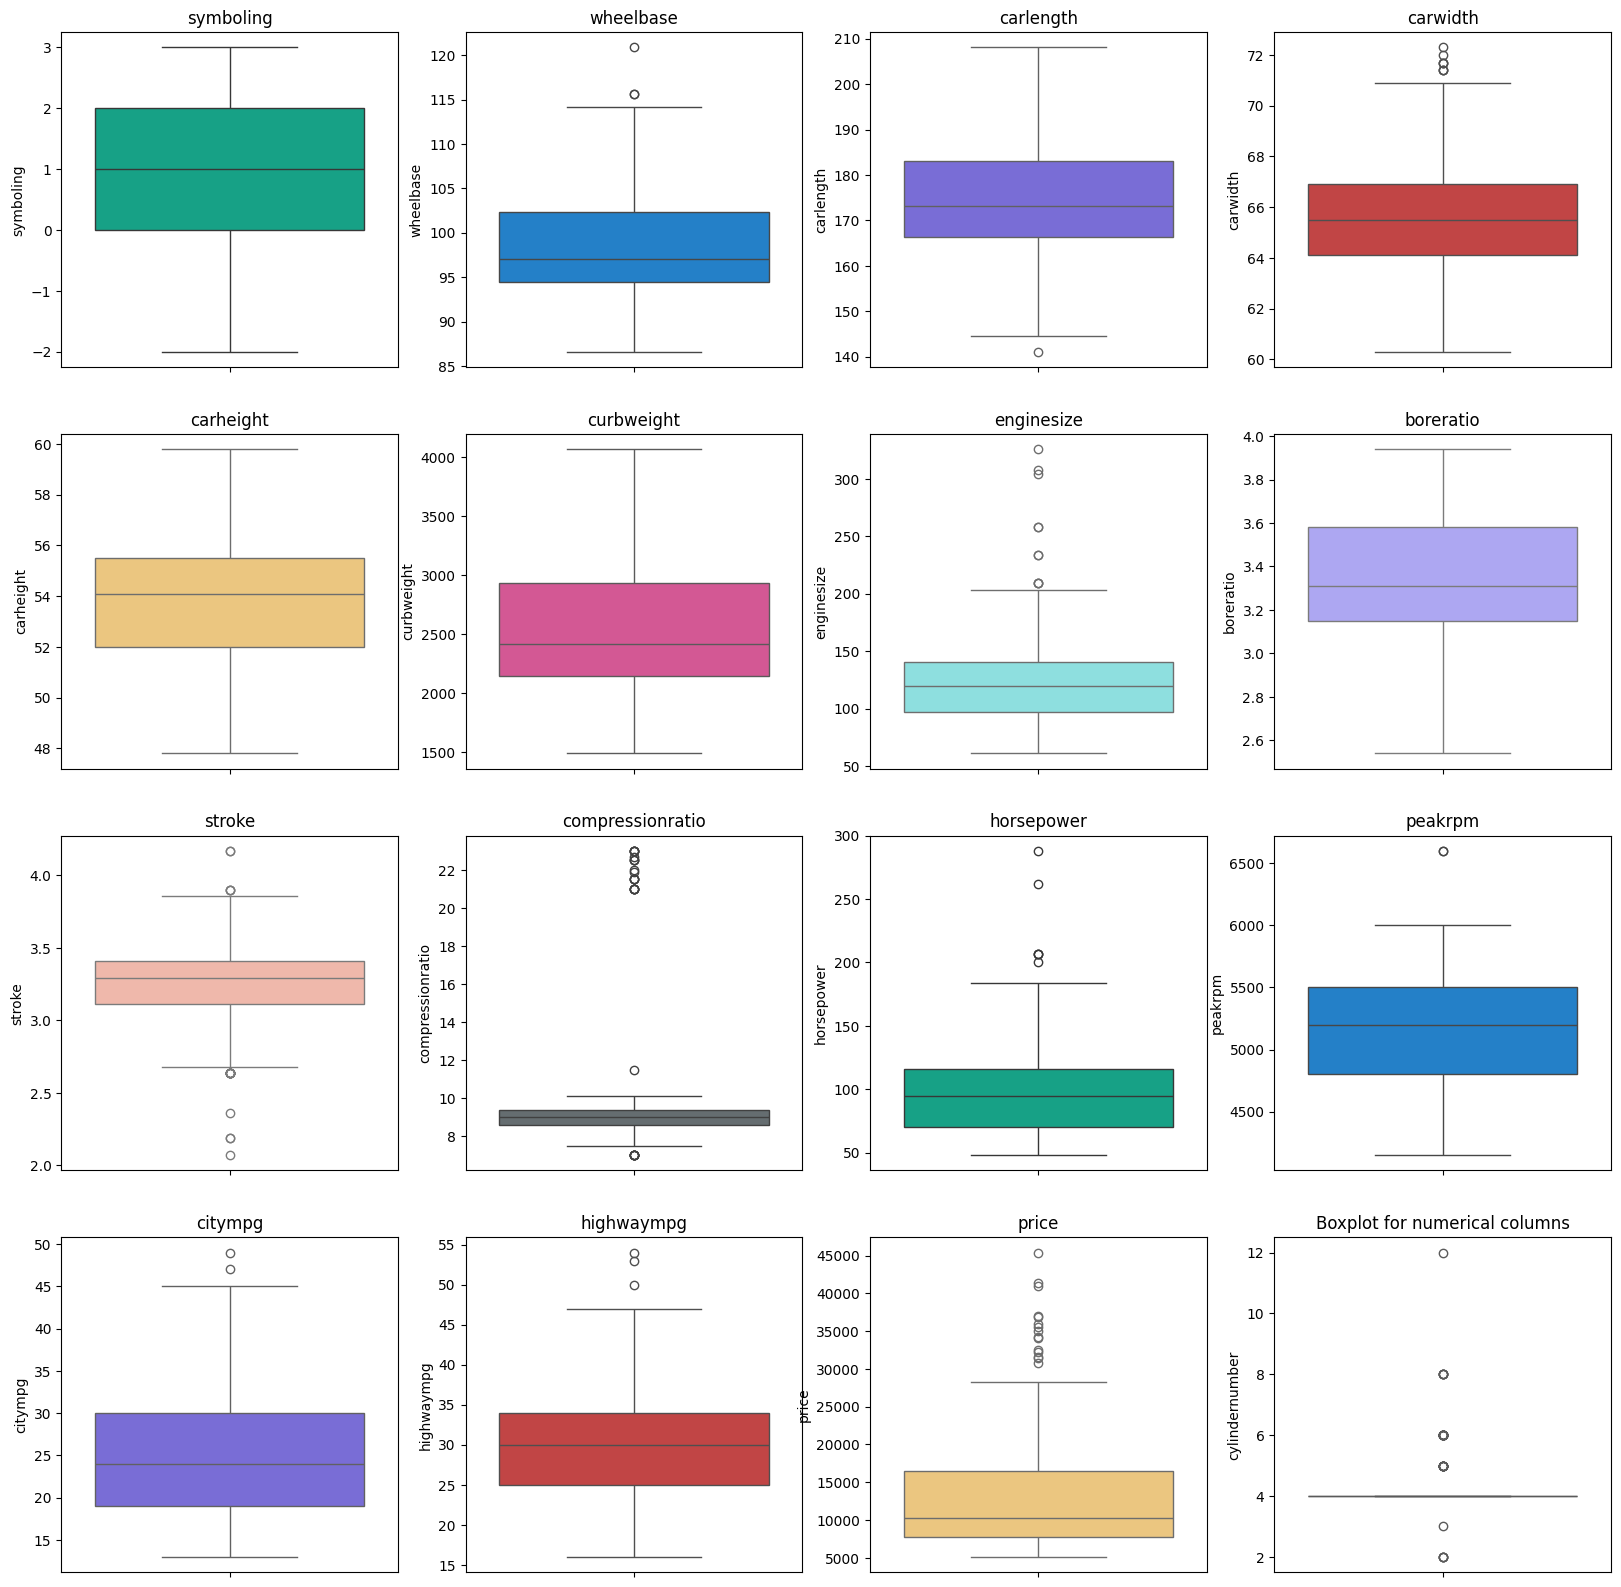
\includegraphics[width=1.0\linewidth]{./figures/data2.png}
        % \captionsetup{labelformat=empty,skip=-8pt}
        % \caption{Early-stage Training in \SB.}
        \label{fig:boxplot}
        \vspace{-5pt}
    \end{subfigure}
    \caption{Data distribution and boxplot.}
    \label{fig:Boxplot}
    \vspace{-12pt}
 \end{figure}
 



\subsubsection{Normalization of Numerical Features}
To eliminate the influence of different scales in numerical features, all numerical attributes were standardized.
Since we notice quite a number of the numerical attributes in this dataset barely follow a normal distribution, MinMaxScalar is favored instead of StandardScalar.
Actually, a much better performance with minmaxscalar is observed in subsequent result.
This transformation helps reserve the distribution and relative distance of the origin data and ensures that the numerical attributes are within [0,1].
The {MinMaxScaler} transformation is defined as:
\[
    x' = \frac{x - x_{\min}}{x_{\max} - x_{\min}},
\]
where $x_{\min}$ and $x_{\max}$ are the minimum and maximum values of the attribute, respectively. This transformation maps all values of $x$ to the range $[0, 1]$.

\subsection{Feature Selection}
After preprocessing, the next step is to identify the most relevant features for clustering. We begin by visualizing the correlation between numerical features using a heatmap, where the correlation coefficient \( r \) between two features \( x_i \) and \( x_j \) is computed as:
$$
r(x_i, x_j) = \frac{\text{cov}(x_i, x_j)}{\sigma_{x_i} \sigma_{x_j}}
$$
where \( \text{cov}(x_i, x_j) \) is the covariance of the features and \( \sigma_{x_i} \) and \( \sigma_{x_j} \) are their respective standard deviations.
Features with high correlation (\( |r| > 0.85 \)) were considered redundant and removed.




\subsubsection{Dimensionality Reduction}
We applied two methods for dimensionality reduction: Principal Component Analysis (PCA) and AutoEncoders (AE). Both methods aim to reduce the number of features while retaining as much variance (PCA) or meaningful information (AE) as possible.

\subsubsection{Principal Component Analysis (PCA)}
PCA~\citep{pearson1901pca,hotelling1933pca} is a linear dimensionality reduction technique that projects the data into a new space such that the first principal component captures the maximum variance in the data, the second principal component captures the second largest variance, and so on. Mathematically, PCA involves solving the eigenvalue problem for the covariance matrix \( \mathbf{C} \) of the dataset:
$$
\mathbf{C} \mathbf{v}_i = \lambda_i \mathbf{v}_i
$$
where \( \lambda_i \) are the eigenvalues and \( \mathbf{v}_i \) are the eigenvectors. 
We selected the number of principal components such that the cumulative explained variance was 95\%.
This resulted in approximately 18 principal components for our dataset, which were used for further analysis.

\subsubsection{AutoEncoder (AE)}
AutoEncoders~\citep{hinton2006autoencoder,goodfellow2016deep} are a class of artificial neural networks that aim to learn a compressed, low-dimensional representation of the input data. The AE consists of an encoder network that maps the input data \( x \) to a lower-dimensional space \( z \), and a decoder network that reconstructs the original data from this lower-dimensional representation. The objective of training an AE is to minimize the reconstruction error:
$$
\mathcal{L}(\hat{x}, x) = \| \hat{x} - x \|^2
$$
For our dataset, we empirically chose the hidden space dimension to match the number of components from PCA (i.e., 20). The architecture and hyperparameters of the AE, including the number of layers and neurons, are summarized in~\autoref{tab:hyperparameter}.



\begin{figure}[!t]
   \centering
   \begin{subfigure}{.32\textwidth}  % Adjust width to fit within the line
       \centering
       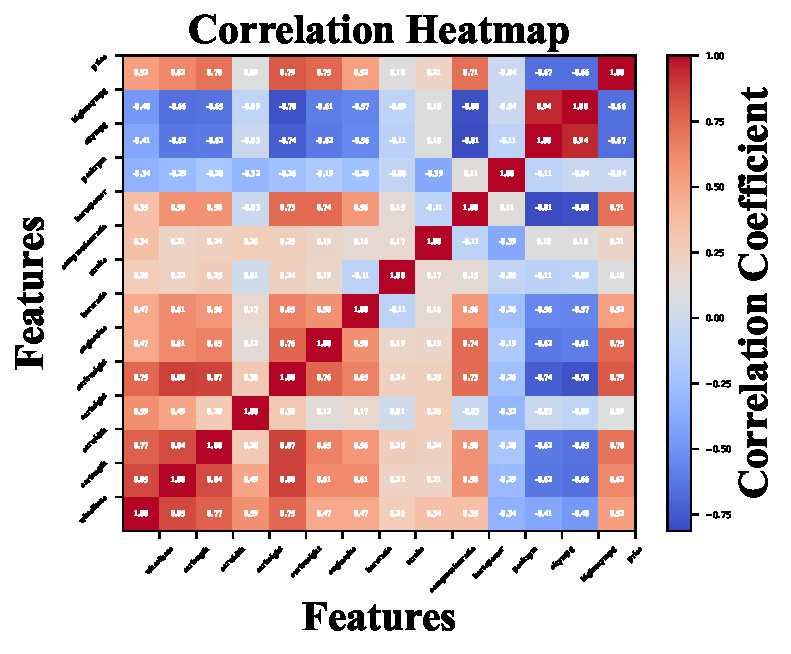
\includegraphics[width=1.0\linewidth]{./figures/correlation_heatmap.pdf}
       % \captionsetup{labelformat=empty,skip=-8pt}
       % \caption{}
       \vspace{-5pt}
       \label{fig:heatmap}
   \end{subfigure}
   \hfill % Ensures that the subfigures are evenly spaced or fill the space
   \begin{subfigure}{.32\textwidth}
       \centering
       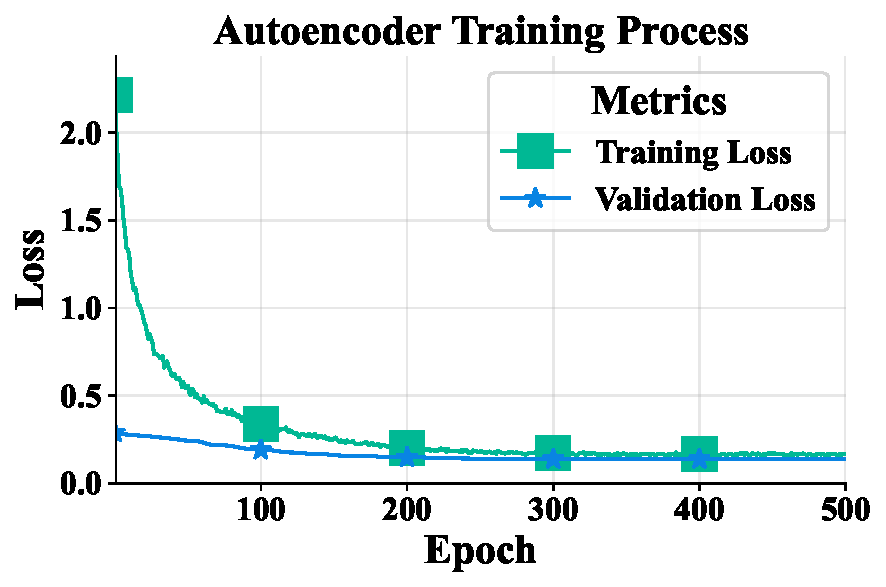
\includegraphics[width=1.0\linewidth]{./figures/autoencoder_training_loss.pdf}
       % \captionsetup{labelformat=empty,skip=-8pt}
       % \caption{}
       \vspace{-5pt}
       \label{fig:loss}
   \end{subfigure}
   \hfill % Use \hfill to add space between subfigures
   \begin{subfigure}{.32\textwidth}
       \centering
       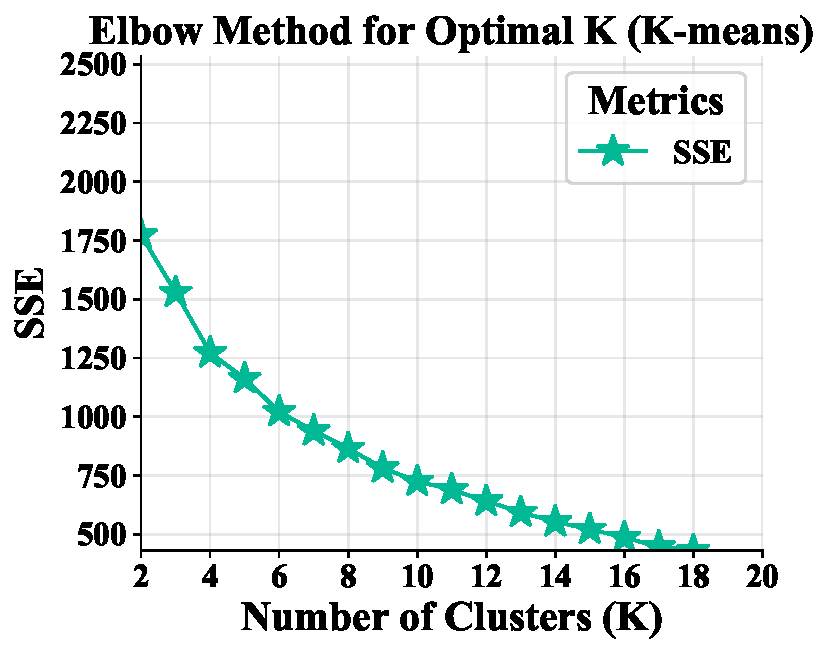
\includegraphics[width=1.0\linewidth]{./figures/elbow_method_deep_kmeans.pdf}
       % \captionsetup{labelformat=empty,skip=-8pt}
       % \caption{}
       \vspace{-5pt}
       \label{fig:elbow}
   \end{subfigure}
   \caption{\textbf{Our propused \textit{Data Selection - Model Training - Application of Clustering Algorithm} Pipeline.} The left figure shows the heatmap of correlations between different data points in the raw data. Middle figure shows the change in the autoencoder loss across training epochs, while the rightmost figure illustrates the process of selecting the optimal parameter K for clustering. And in this problem, we choose K=8.}
   \vspace{-10pt}
   \label{fig:pipeline}
\end{figure}



\begin{table}[ht]
   \centering
   \begin{tabular}{lc}
   \toprule
   \textbf{Hyperparameter} & \textbf{Value} \\ \midrule
   Active Function & ReLU \\
   Encoding Dimension & 20 \\
   Number of Layers & 7 \\
   Batch Size & 128 \\
   Epochs & 500 \\
   Learning Rate & 1e-3 \\
   Loss Function & MSE \\
   Optimizer & Adam \\
   Dropout Rate & 0.2 \\
   \bottomrule
   \end{tabular}
   \caption{Autoencoder Architecture and Hyperparameters}
   \label{tab:hyperparameter}
\end{table}



\subsection{Clustering Algorithms}
After reducing the feature space to approximately 20 dimensions, we applied two clustering methods to identify groups of similar vehicles: K-means and hierarchical clustering.

\subsubsection{K-means Clustering}
K-means clustering~\citep{macqueen1967kmeans,jain2010kmeans} is a centroid-based clustering algorithm that partitions the dataset into \( K \) clusters, where each data point belongs to the cluster whose centroid is nearest. The objective is to minimize the within-cluster sum of squared errors (SSE):
$$
SSE(K) = \sum_{i=1}^{N} \sum_{k=1}^{K} \mathbf{1}(c_i=k) \| x_i - \mu_k \|^2
$$
where \( c_i \) is the cluster assignment for data point \( x_i \), \( \mu_k \) is the centroid of cluster \( k \), and \( \mathbf{1}(\cdot) \) is the indicator function. To determine the optimal number of clusters \( K \), we used the elbow method, plotting the SSE as a function of \( K \) and selecting the \( K \) where the rate of decrease in SSE starts to slow,
as shown in~\figref{fig:pipeline}.

\subsubsection{Hierarchical Clustering}
Hierarchical clustering~\citep{lance1967hierarchical,murtagh2012hierarchical} builds a tree of clusters by either iteratively merging smaller clusters (agglomerative) or splitting larger clusters (divisive). The agglomerative approach was used for this problem, where at each step, the two clusters that are closest according to a chosen distance metric are merged. The proximity between clusters can be measured using various linkage criteria, such as single linkage, complete linkage, or average linkage. The distance between two clusters \( A \) and \( B \) is given by:
$$
d(A, B) = \min_{x \in A, y \in B} \| x - y \|
$$
We used a dendrogram to visually inspect the hierarchical relationships between the clusters, as shown in~\autoref{fig:dendrogram}, then we selected the appropriate number of clusters based on the structure of the tree. For this problem, we finally choose 8 clusters (Distance around 10).




\begin{figure}[!t]
   \centering
   % \includegraphics[width=1.0\linewidth]{resources/figures/strategy.pdf}
   \begin{subfigure}{.49\textwidth}  % Adjust width to fit within the line
       \centering
       % \framebox[\linewidth][c]{\phantom{\rule{0pt}{0.918\linewidth}}}
       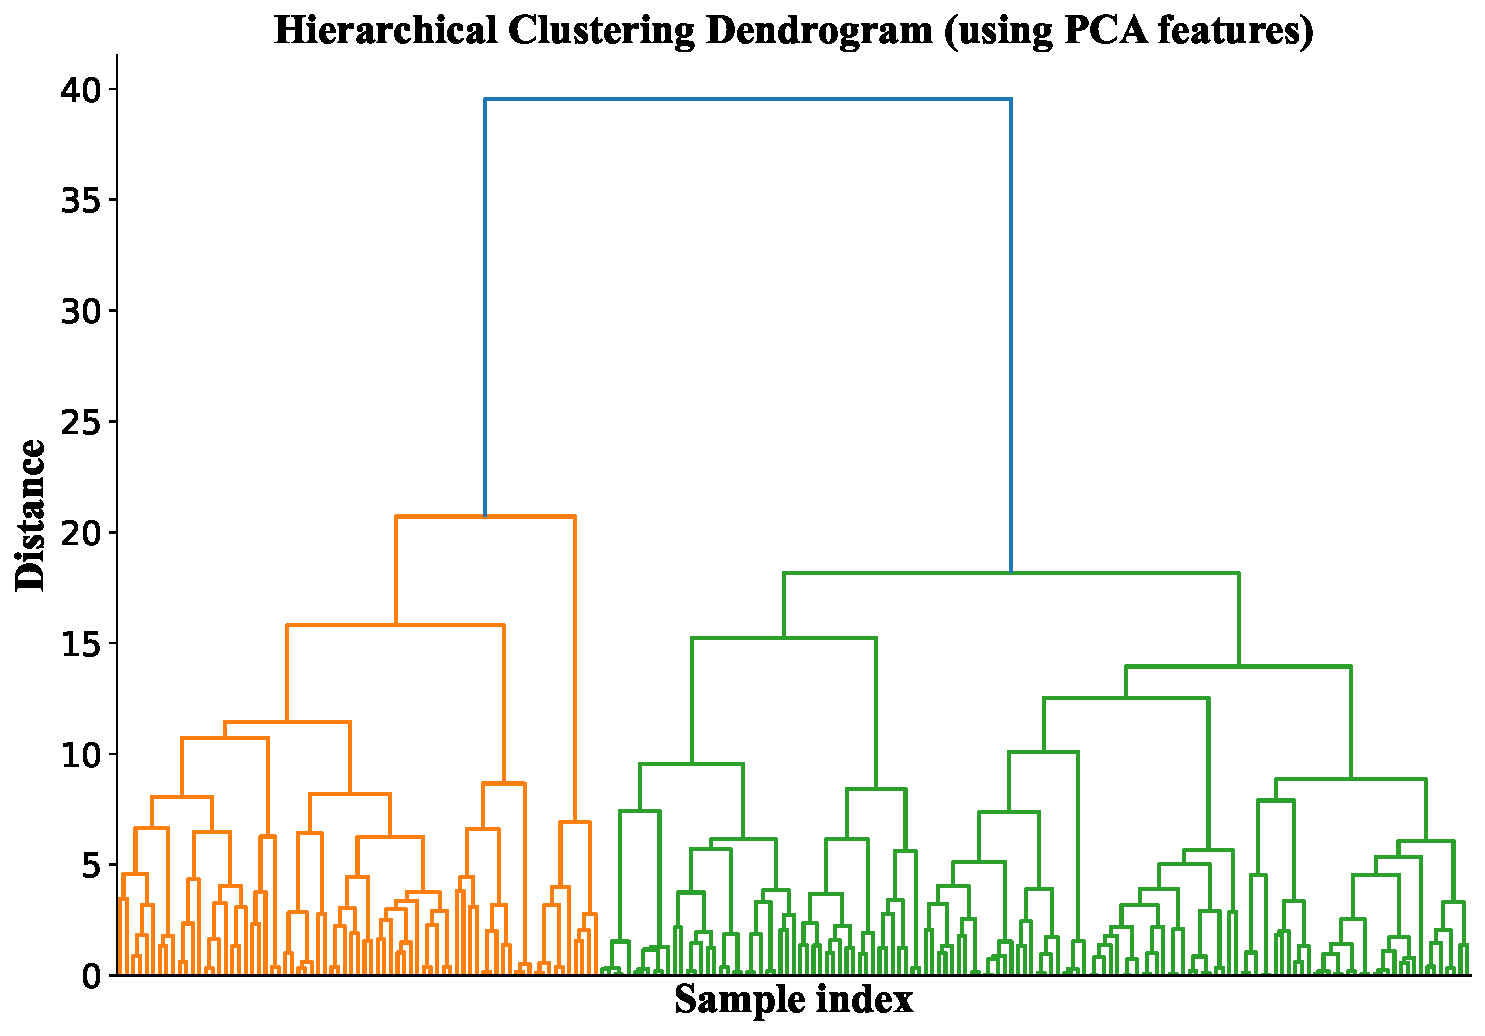
\includegraphics[width=1.0\linewidth]{./figures/hierarchical_dendrogram.pdf}
       % \captionsetup{labelformat=empty,skip=-8pt}
       % \caption{Comparison \SA and \SB.}
       \vspace{-5pt}
       \label{fig:dendrogram1}
   \end{subfigure}
   \hfill % Ensures that the subfigures are evenly spaced or fill the space
   \begin{subfigure}{.49\textwidth}
       \centering
       % \framebox[\linewidth][c]{\phantom{\rule{0pt}{0.918\linewidth}}}
       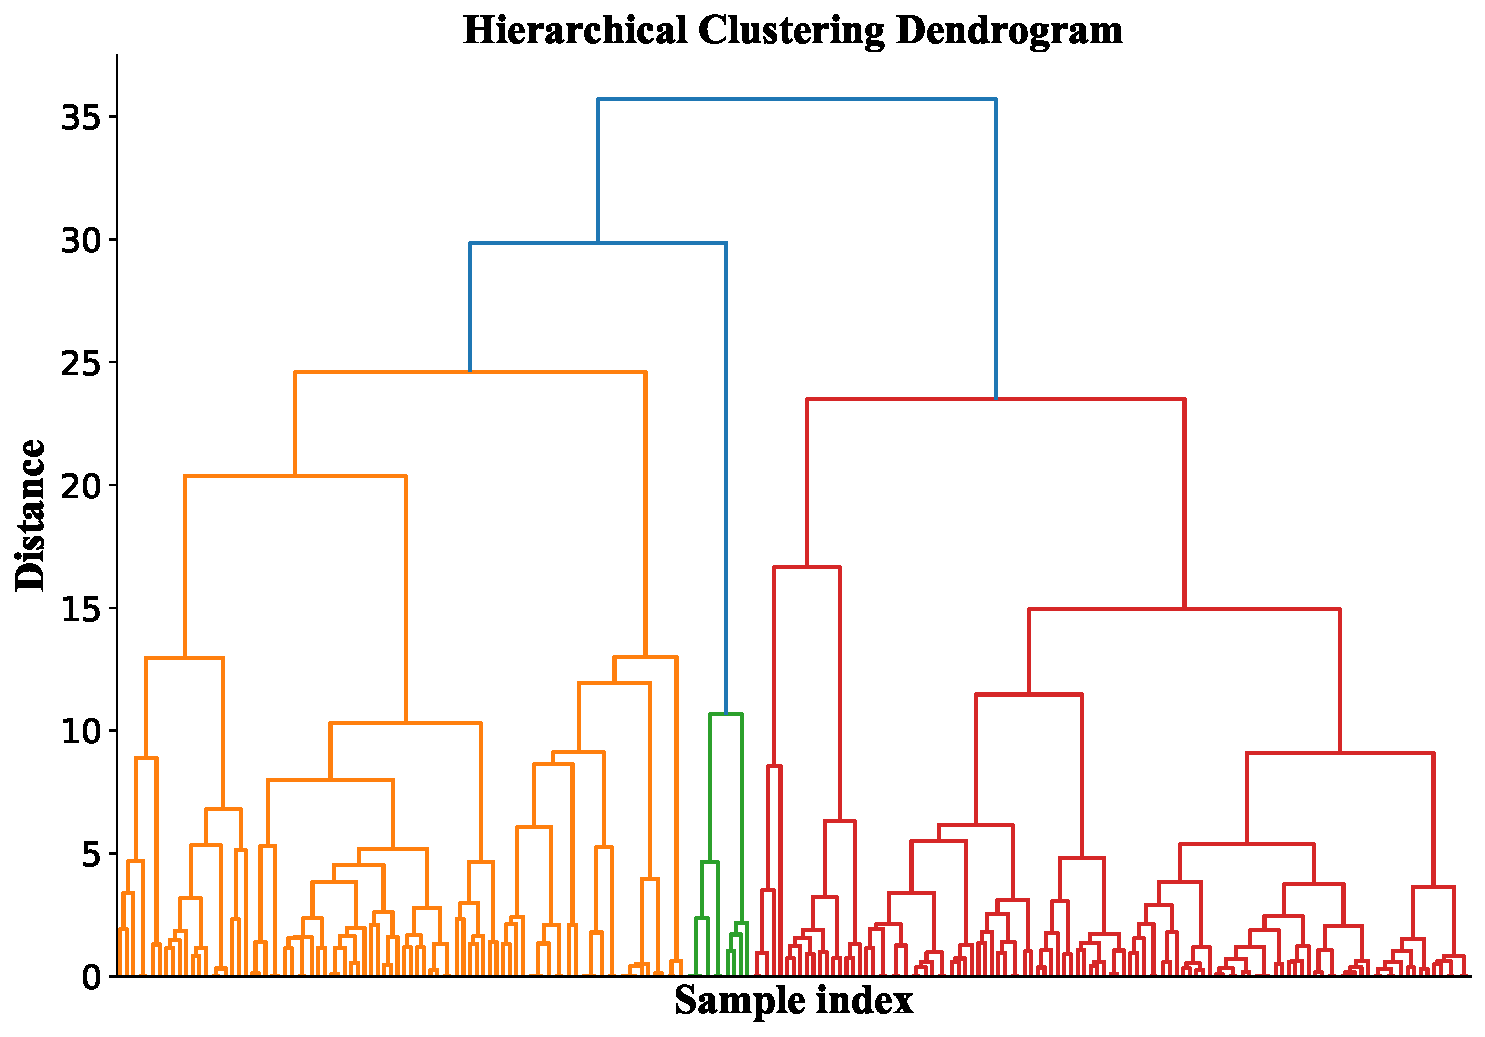
\includegraphics[width=1.0\linewidth]{./figures/hierarchical_dendrogram_deep.pdf}
       % \captionsetup{labelformat=empty,skip=-8pt}
       % \caption{Early-stage Training in \SB.}
       \vspace{-5pt}
       \label{fig:dendrogram2}
   \end{subfigure}
   \caption{\textbf{Dendrogram of the Bottom-Up Hierarchical Clustering Process on the Low-Dimensional Features Generated by \textit{PCA} and \textit{AE}.} From the figure, it is evident that a reasonable choice for the number of clusters is around 10, corresponding to a distance of approximately 10.}
   \label{fig:dendrogram}
   \vspace{-12pt}
\end{figure}


\section{Numerical Results}
\label{sec:numerical}

\subsection{Model Evaluation}
To evaluate the performance of the clustering algorithms, we used internal validation metrics in~\autoref{tab:evaluation_metric} in~\autoref{sec:app}\footnote{Due to space limitations and for the sake of aesthetic formatting.}.
The table compares the performance of clustering methods (Kmeans and Hierarchical Clustering, HC) on features extracted using PCA and Autoencoder (AE) across four evaluation metrics: Silhouette Score(SC)~\citep{rousseeuw1987silhouettes}, Calinski-Harabasz Index(CH)~\citep{calinski1974dendrite}, Davies-Bouldin Index(DB)~\citep{davies1979cluster} and Dunn Index(DI)~\citep{dunn1974well}.



\subsection{Clustering results}
For the clustering results, see~\autoref{fig:visual}, Tabel~\ref{tab:cluster_PCA_kmeans},\ref{tab:cluster_AE_kmeans},\ref{tab:cluster_PCA_hc} and \ref{tab:cluster_AE_hc} in~\autoref{sec:app}.
Based on the results of the five tables, we find that \purpletext{for feature extraction, Autoencoder (AE) outperforms Principal Component Analysis (PCA) in terms of clustering quality}. 
For example, AE combined with hierarchical clustering (HC) yields the best SC (0.3864) and DB (1.0059), suggesting that this method effectively separates data points.

In the clustering methods, K-means slightly outperforms HC when using AE features, achieving a higher CH score. However, HC with PCA features achieves the highest Dunn Index (DI) score (0.3674), suggesting that it can identify well-separated clusters despite its lower SC and CH.

Examining the cluster composition, AE-based features result in a more meaningful distribution of vehicles across clusters, with distinct median prices and a better grouping of VW vehicles. For example, clusters generated with AE features using K-means place most VW vehicles in clusters with moderate median prices (e.g., $9,717.14$ and $10,445$), aligning with VW's market position. In contrast, PCA-based clusters show less consistent grouping, with VW vehicles distributed across multiple clusters without clear price patterns.

Overall, the combination of AE for feature extraction and HC for clustering not only achieves the best clustering evaluation metrics but also results in a logical grouping of vehicles that reflects market segmentation. 
And we use this result (i.e. \purpletext{AE+HC}) for next sections's analysis.

\begin{figure}[!t]
    \centering
    % \includegraphics[width=1.0\linewidth]{resources/figures/strategy.pdf}
    \begin{subfigure}{.24\textwidth}  % Adjust width to fit within the line
        \centering
        % \framebox[\linewidth][c]{\phantom{\rule{0pt}{0.918\linewidth}}}
        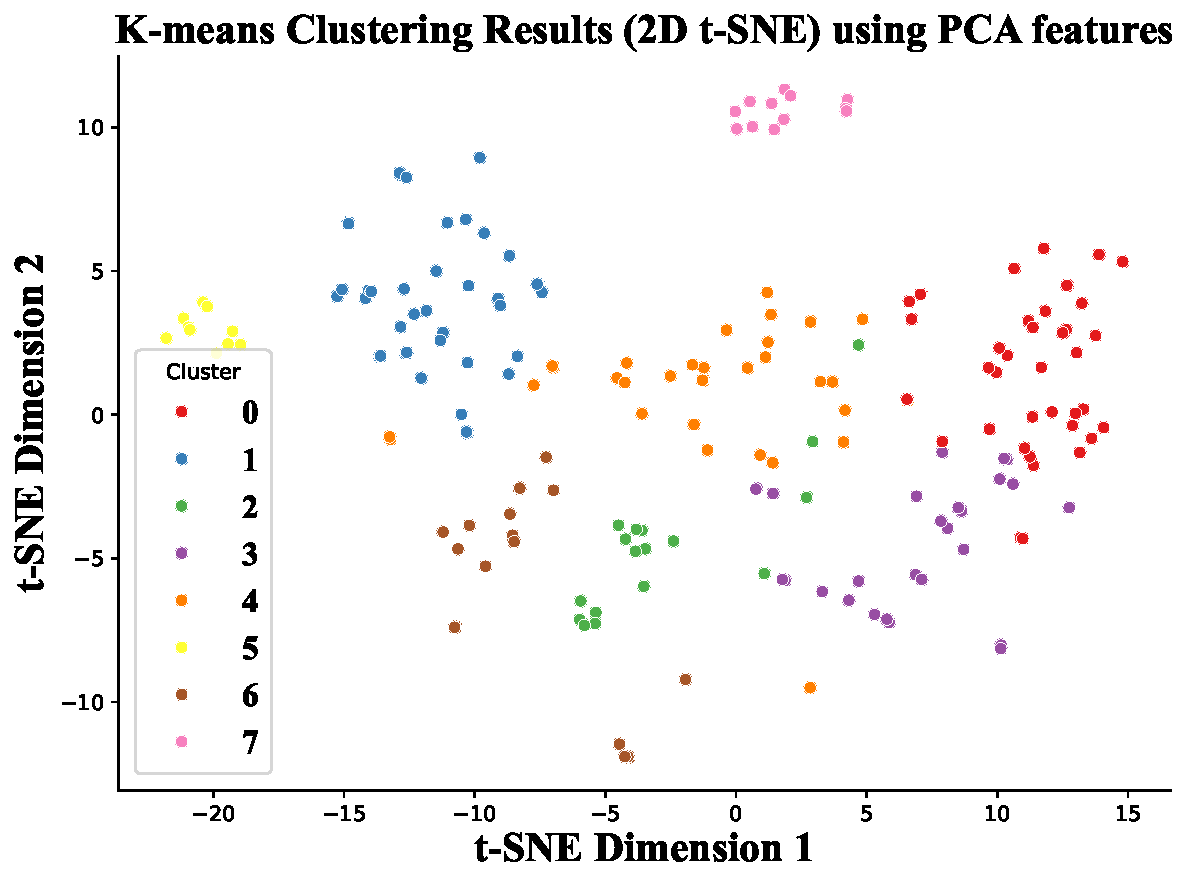
\includegraphics[width=1.0\linewidth]{./figures/PCA_kmeans_tsne_2d.pdf}
        % \captionsetup{labelformat=empty,skip=-8pt}
        % \caption{Comparison \SA and \SB.}
        \vspace{-5pt}
        \label{fig:visual1}
    \end{subfigure}
    \hfill % Ensures that the subfigures are evenly spaced or fill the space
    \begin{subfigure}{.24\textwidth}
        \centering
        % \framebox[\linewidth][c]{\phantom{\rule{0pt}{0.918\linewidth}}}
        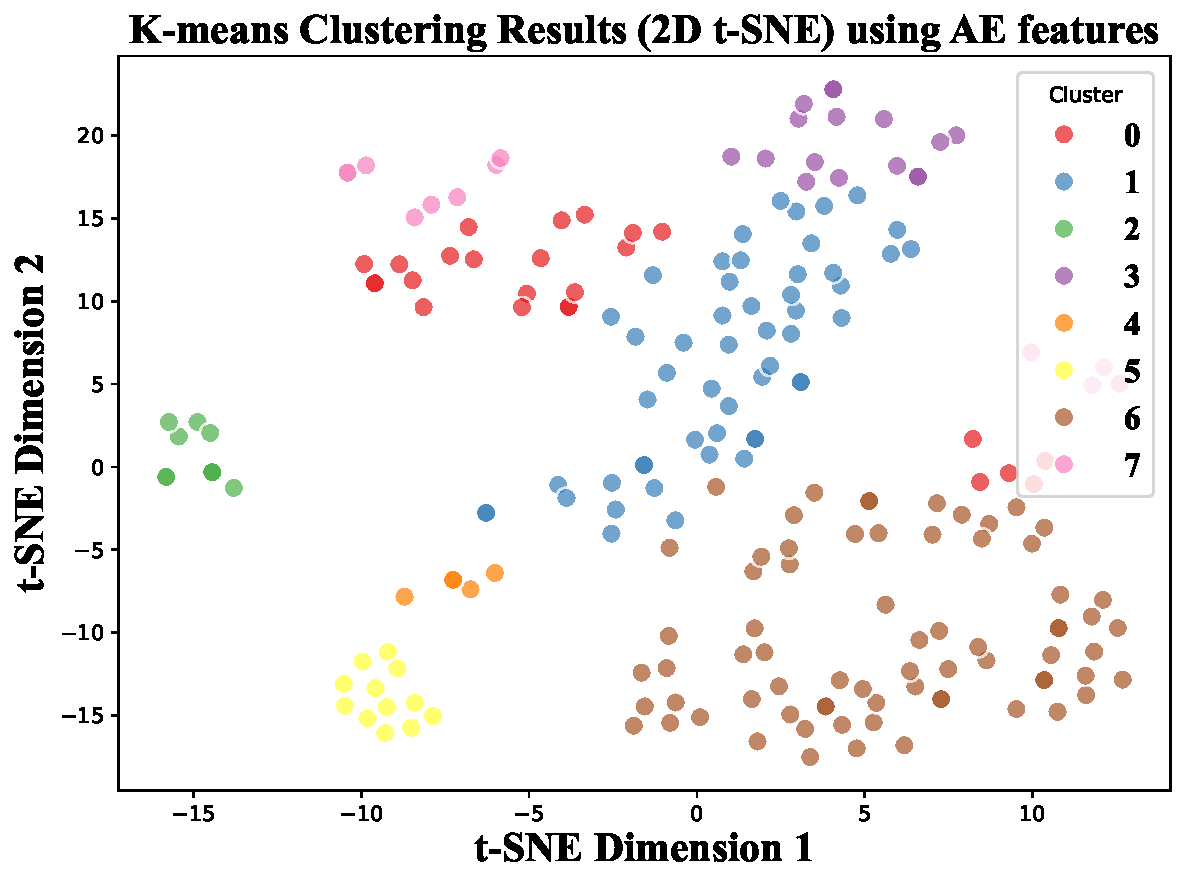
\includegraphics[width=1.0\linewidth]{./figures/AE_kmeans_tsne_2d.pdf}
        % \captionsetup{labelformat=empty,skip=-8pt}
        % \caption{Early-stage Training in \SB.}
        \vspace{-5pt}
        \label{fig:visual2}
    \end{subfigure}
    \hfill % Ensures that the subfigures are evenly spaced or fill the space
    \begin{subfigure}{.24\textwidth}
        \centering
        % \framebox[\linewidth][c]{\phantom{\rule{0pt}{0.918\linewidth}}}
        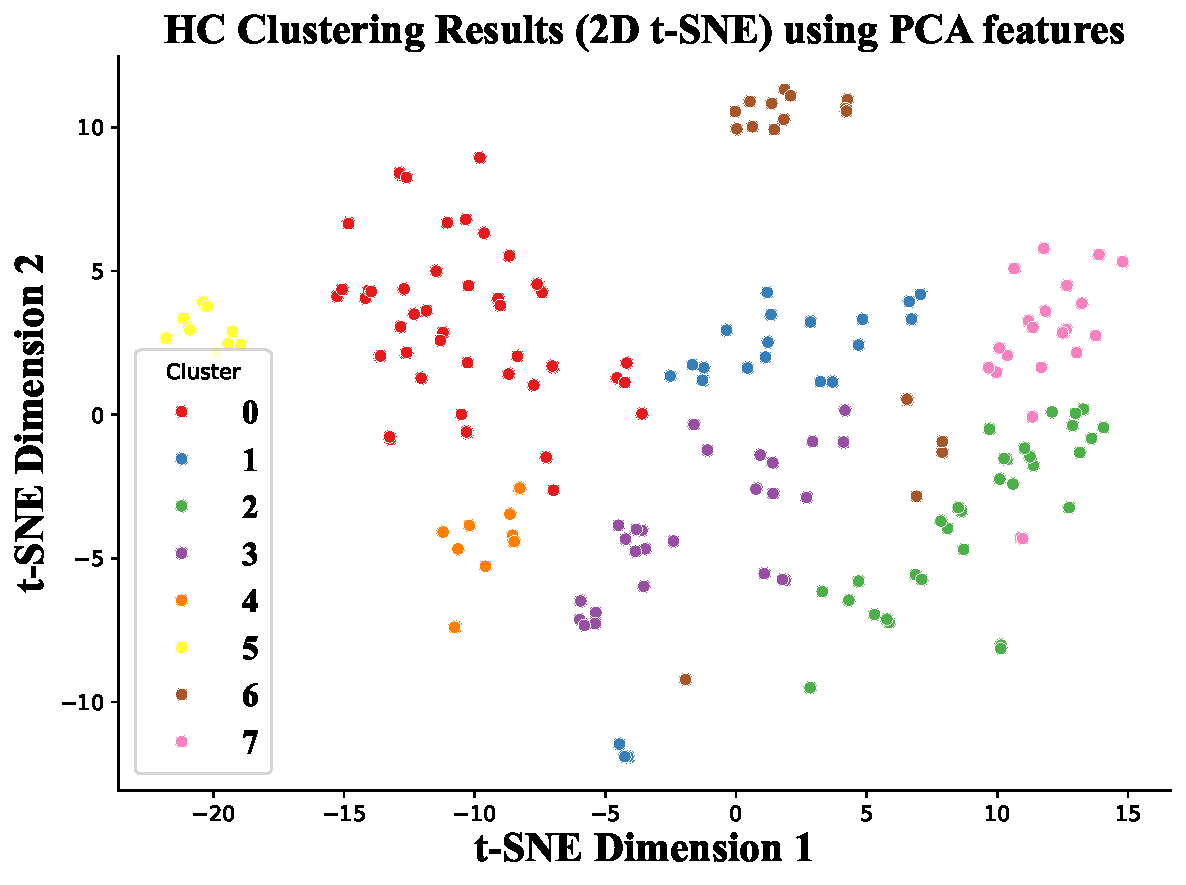
\includegraphics[width=1.0\linewidth]{./figures/PCA_hc_tsne_2d.pdf}
        % \captionsetup{labelformat=empty,skip=-8pt}
        % \caption{Early-stage Training in \SB.}
        \vspace{-5pt}
        \label{fig:visual3}
    \end{subfigure}
    \hfill % Ensures that the subfigures are evenly spaced or fill the space
    \begin{subfigure}{.24\textwidth}
        \centering
        % \framebox[\linewidth][c]{\phantom{\rule{0pt}{0.918\linewidth}}}
        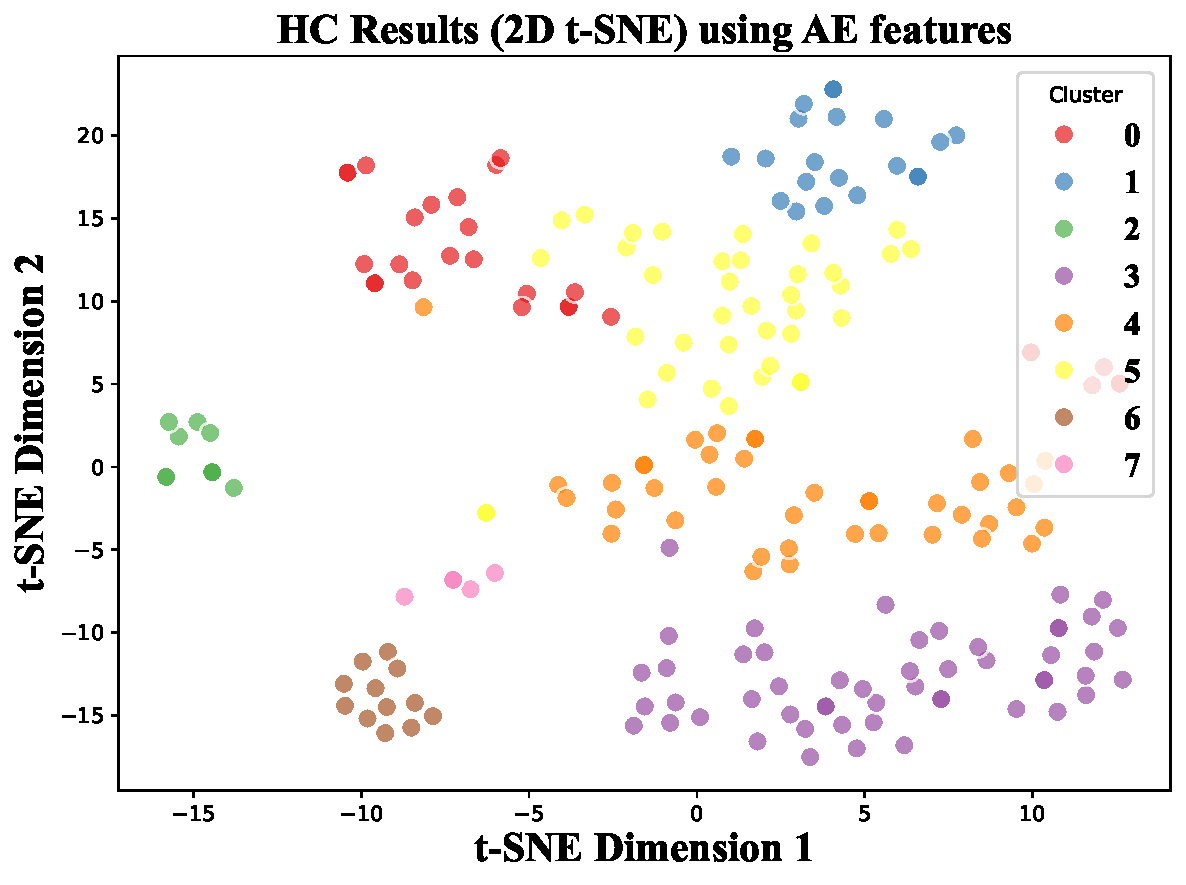
\includegraphics[width=1.0\linewidth]{./figures/AE_hc_tsne_2d.pdf}
        % \captionsetup{labelformat=empty,skip=-8pt}
        % \caption{Early-stage Training in \SB.}
        \vspace{-5pt}
        \label{fig:visual4}
    \end{subfigure}
 
    \caption{\textbf{2D Visualization of Features Generated by \textit{Kmeans} and \textit{Hierarchical Clustering} after Dimensionality Reduction Using \textit{PCA} and \textit{AE}.} The clustering results are visually clearer when using \textit{AE} for dimensionality reduction, as samples within the same cluster are more densely packed.}
    \label{fig:visual}
    \vspace{-12pt}
 \end{figure}
 
 


\section{Conclusion}
\label{sec:conclusion}

We selected cars that \bluetext{\textit{belong to the same cluster as Volkswagen vehicles and have prices within 10\% of the average price of Volkswagen vehicles}} as the final competitor models
and provide the competitors in the .csv files in our \texttt{Supplementary materials}, please refer to \greentext{cars\_within\_10\_percent.csv}.
And we further analysis the attributes of the cars after clustering, as shown in~\autoref{fig:combined_analysis} in~\autoref{sec:app}.

According to these figures. The competitors of Volkswagen share several characteristics that align with the positioning of affordable and practical urban vehicles. These models typically fall into the sedan or hatchback categories, emphasizing compactness and maneuverability, making them well-suited for city driving.
Furthermore, these vehicles are generally offered at a lower price point, appealing to cost-sensitive consumers who prioritize economic value over premium features. Their fuel efficiency, reflected in high city and highway mileage, further solidifies their appeal to urban drivers.

However, there are notable differences that set Volkswagen apart from its competitors. Many competing models prioritize lightweight construction, which, while beneficial for fuel efficiency, may compromise perceived safety and structural integrity. In contrast, Volkswagen is often recognized for its robust build and focus on safety, offering a significant edge in terms of quality assurance. 
Moreover, the competitors’ emphasis on fuel efficiency often results in lower engine power, with many models delivering modest horsepower. Volkswagen, on the other hand, strives to strike a balance between performance and efficiency, catering to drivers who value a more dynamic driving experience.
Another area of differentiation lies in interior design and comfort. Competitors frequently offer smaller cabin dimensions, which may suffice for short urban commutes but could reduce comfort on longer journeys. 







\bibliography{iclr2025_conference}
\bibliographystyle{iclr2025_conference}


\vspace{4cm}
\appendix
\section{Appendix}
\label{sec:app}


% \vspace{-2cm}
\begin{table}[H]
    \centering
    \begin{tabular}{c|c|>{\centering\arraybackslash}p{1.5cm}|>{\centering\arraybackslash}p{1.5cm}|>{\centering\arraybackslash}p{1.5cm}|>{\centering\arraybackslash}p{1.5cm}}
        \toprule
        \multirow{2}{*}{\textbf{Feature}} & \multirow{2}{*}{\textbf{Cluster}} & \multicolumn{4}{c}{\textbf{Evaluation Metric}} \\
        \cmidrule(lr){3-6}
                                       &                                & \textbf{SC} & \textbf{CH} & \textbf{DB} & \textbf{DI} \\
        \midrule
        \multirow{2}{*}{PCA}           & Kmeans                         &        0.2093     &      29.9797       &      1.6294       &     0.2707        \\
                                       & \cellcolor{gray!20} HC                             & \cellcolor{gray!20} 0.2010 & \cellcolor{gray!20}  28.0231& \cellcolor{gray!20} 1.6160 & \cellcolor{gray!20} \textbf{0.3674 $\uparrow$} \\
        \midrule
        \multirow{2}{*}{AE}            & Kmeans                         &       0.3746      &      \textbf{78.2700 $\uparrow$}       &     1.0583        &   0.0867          \\
                                       &\cellcolor{gray!20} HC                             & \cellcolor{gray!20} \textbf{0.3864 $\uparrow$}  & \cellcolor{gray!20} 75.5768 & \cellcolor{gray!20} \textbf{1.0059 $\downarrow$} & \cellcolor{gray!20} 0.1957 \\
        \bottomrule
    \end{tabular}
    \caption{Clustering Methods and Evaluation Metrics.}% For PCA-based features, Kmeans outperforms HC on SC, CH, and DB metrics, indicating better compactness and separation of clusters. 

    \label{tab:evaluation_metric}
 \end{table}
 
 \kern -0.5cm 



 \begin{table}[H]
    \setlength{\extrarowheight}{2pt} % 减少行间距
    \centering
    \begin{tabular}{l|>{\centering\arraybackslash}p{1cm}|>{\centering\arraybackslash}p{1cm}|>{\centering\arraybackslash}p{1cm}|>{\centering\arraybackslash}p{1cm}|>{\centering\arraybackslash}p{1cm}|>{\centering\arraybackslash}p{1cm}|>{\centering\arraybackslash}p{1cm}|>{\centering\arraybackslash}p{1cm}}
        \toprule
        \textbf{} & \multicolumn{8}{c}{\textbf{K-means Cluster (PCA feature)}} \\
        \cmidrule(lr){2-9}
        \textbf{} & \textbf{0} & \textbf{1} & \textbf{2} & \textbf{3} & \textbf{4} & \textbf{5} & \textbf{6} & \textbf{7} \\
        \midrule
        \textbf{Number of cars} & 21 & 46 & 35 & 21 & 27 & 25 & 18 & 12 \\
        \textbf{Median price}   & \cellcolor{gray!20}11541 & \cellcolor{gray!20}8279 & \cellcolor{gray!20}6817 & \cellcolor{gray!20}14670 & \cellcolor{gray!20}22163 & \cellcolor{gray!20}12175 & \cellcolor{gray!20}22326 & \cellcolor{gray!20}20602 \\
        \textbf{Number of VW}   & 2 & 1 & 0 & 0 & 0 & 8 & 0 & 1 \\
        \textbf{VW Median}      & \cellcolor{gray!20}10788 & \cellcolor{gray!20}12290 & \cellcolor{gray!20} - & \cellcolor{gray!20}- & \cellcolor{gray!20}- & \cellcolor{gray!20}9153 & \cellcolor{gray!20}- & \cellcolor{gray!20}13845 \\
        \bottomrule
    \end{tabular}
    \caption{K-means clusters using PCA features}
    \label{tab:cluster_PCA_kmeans}
\end{table}

\kern -0.5cm 

\begin{table}[H]
    \setlength{\extrarowheight}{2pt} % 减少行间距
    \centering
    \begin{tabular}{l|>{\centering\arraybackslash}p{1cm}|>{\centering\arraybackslash}p{1cm}|>{\centering\arraybackslash}p{1cm}|>{\centering\arraybackslash}p{1cm}|>{\centering\arraybackslash}p{1cm}|>{\centering\arraybackslash}p{1cm}|>{\centering\arraybackslash}p{1cm}|>{\centering\arraybackslash}p{1cm}}
        \toprule
        \textbf{} & \multicolumn{8}{c}{\textbf{K-means Cluster (AE feature)}} \\
        \cmidrule(lr){2-9}
        \textbf{} & \textbf{0} & \textbf{1} & \textbf{2} & \textbf{3} & \textbf{4} & \textbf{5} & \textbf{6} & \textbf{7} \\
        \midrule
        \textbf{Number of cars} & 27 & 44 & 17 & 39 & 50 & 14 & 11 & 3 \\
        \textbf{Median price}   & \cellcolor{gray!20}21624 & \cellcolor{gray!20}15348 & \cellcolor{gray!20}7428 & \cellcolor{gray!20}7862 & \cellcolor{gray!20}9843 & \cellcolor{gray!20}17659 & \cellcolor{gray!20}23079 & \cellcolor{gray!20}12145 \\
        \textbf{Number of VW}   & 0 & 2 & 0 & 0 & 7 & 3 & 0 & 0 \\
        \textbf{VW Median}      & \cellcolor{gray!20}- & \cellcolor{gray!20}10788 & \cellcolor{gray!20}- & \cellcolor{gray!20}- & \cellcolor{gray!20}9717 & \cellcolor{gray!20}10445 & \cellcolor{gray!20}- & \cellcolor{gray!20}- \\
        \bottomrule
    \end{tabular}
    \caption{K-means clusters using AE features}
    \label{tab:cluster_AE_kmeans}
\end{table}

\kern -0.5cm 

\begin{table}[H]
    \setlength{\extrarowheight}{2pt} % 减少行间距
    \centering
    \begin{tabular}{l|>{\centering\arraybackslash}p{1cm}|>{\centering\arraybackslash}p{1cm}|>{\centering\arraybackslash}p{1cm}|>{\centering\arraybackslash}p{1cm}|>{\centering\arraybackslash}p{1cm}|>{\centering\arraybackslash}p{1cm}|>{\centering\arraybackslash}p{1cm}|>{\centering\arraybackslash}p{1cm}}
        \toprule
        \textbf{} & \multicolumn{8}{c}{\textbf{Hierarchical Cluster (PCA feature)}} \\
        \cmidrule(lr){2-9}
        \textbf{} & \textbf{0} & \textbf{1} & \textbf{2} & \textbf{3} & \textbf{4} & \textbf{5} & \textbf{6} & \textbf{7} \\
        \midrule
        \textbf{Number of cars} & 47 & 25 & 21 & 38 & 19 & 20 & 16 & 19 \\
        \textbf{Median price}   & \cellcolor{gray!20}7004 & \cellcolor{gray!20}15092 & \cellcolor{gray!20}15934 & \cellcolor{gray!20}8816 & \cellcolor{gray!20}13251 & \cellcolor{gray!20}18938 & \cellcolor{gray!20}11608 & \cellcolor{gray!20}27859 \\
        \textbf{Number of VW}   & 0 & 0 & 4 & 1 & 5 & 0 & 2 & 0 \\
        \textbf{VW Median}      & \cellcolor{gray!20}- & \cellcolor{gray!20}- & \cellcolor{gray!20}9778 & \cellcolor{gray!20}12290 & \cellcolor{gray!20}9591 & \cellcolor{gray!20}- & \cellcolor{gray!20}10788 & \cellcolor{gray!20}- \\
        \bottomrule
    \end{tabular}
    \caption{Hierarchical clusters using PCA features}
    \label{tab:cluster_PCA_hc}
\end{table}

\kern -0.5cm 

\begin{table}[H]
    \setlength{\extrarowheight}{2pt} % 减少行间距
    \centering
    \begin{tabular}{l|>{\centering\arraybackslash}p{1cm}|>{\centering\arraybackslash}p{1cm}|>{\centering\arraybackslash}p{1cm}|>{\centering\arraybackslash}p{1cm}|>{\centering\arraybackslash}p{1cm}|>{\centering\arraybackslash}p{1cm}|>{\centering\arraybackslash}p{1cm}|>{\centering\arraybackslash}p{1cm}}
        \toprule
        \textbf{} & \multicolumn{8}{c}{\textbf{Hierarchical Cluster (AE feature)}} \\
        \cmidrule(lr){2-9}
        \textbf{} & \textbf{0} & \textbf{1} & \textbf{2} & \textbf{3} & \textbf{4} & \textbf{5} & \textbf{6} & \textbf{7} \\
        \midrule
        \textbf{Number of cars} & 61 & 13 & 52 & 17 & 14 & 28 & 3 & 17 \\
        \textbf{Median price}   & \cellcolor{gray!20}9081 & \cellcolor{gray!20}19505 & \cellcolor{gray!20}10559 & \cellcolor{gray!20}18530 & \cellcolor{gray!20}20958 & \cellcolor{gray!20}21216 & \cellcolor{gray!20}12145 & \cellcolor{gray!20}7428 \\
        \textbf{Number of VW}   & 2 & 1 & 9 & 0 & 0 & 0 & 0 & 0 \\
        \textbf{VW Median}      & \cellcolor{gray!20}10788 & \cellcolor{gray!20}9495 & \cellcolor{gray!20}9984 & \cellcolor{gray!20}- & \cellcolor{gray!20}- & \cellcolor{gray!20}- & \cellcolor{gray!20}- & \cellcolor{gray!20}- \\
        \bottomrule
    \end{tabular}
    \caption{Hierarchical clusters using AE features}
    \label{tab:cluster_AE_hc}
\end{table}


% \begin{center}
%     \begin{longtable}{@{}lllr@{}}
%     % \caption{Dataset overview}
%     \toprule
%     \#   & Column             & Non-Null Count & Dtype   \\ \midrule
%     0    & car\_ID            & 205 non-null   & int64   \\
%     1    & symboling          & 205 non-null   & int64   \\
%     2    & CarName            & 205 non-null   & object  \\
%     3    & fueltype           & 205 non-null   & object  \\
%     4    & aspiration         & 205 non-null   & object  \\
%     5    & doornumber         & 205 non-null   & object  \\
%     6    & carbody            & 205 non-null   & object  \\
%     7    & drivewheel         & 205 non-null   & object  \\
%     8    & enginelocation     & 205 non-null   & object  \\
%     9    & wheelbase          & 205 non-null   & float64 \\
%     10   & carlength          & 205 non-null   & float64 \\
%     11   & carwidth           & 205 non-null   & float64 \\
%     12   & carheight          & 205 non-null   & float64 \\
%     13   & curbweight         & 205 non-null   & int64   \\
%     14   & enginetype         & 205 non-null   & object  \\
%     15   & cylindernumber     & 205 non-null   & object  \\
%     16   & enginesize         & 205 non-null   & int64   \\
%     17   & fuelsystem         & 205 non-null   & object  \\
%     18   & boreratio          & 205 non-null   & float64 \\
%     19   & stroke             & 205 non-null   & float64 \\
%     20   & compressionratio   & 205 non-null   & float64 \\
%     21   & horsepower         & 205 non-null   & int64   \\
%     22   & peakrpm            & 205 non-null   & int64   \\
%     23   & citympg            & 205 non-null   & int64   \\
%     24   & highwaympg         & 205 non-null   & int64   \\
%     25   & price              & 205 non-null   & float64 \\ \bottomrule
%     \end{longtable}
%     \label{tab:data}
% \end{center}
    


\begin{figure}[htbp]
    \centering
    % 第一张图
    \begin{subfigure}[b]{\linewidth}
        \centering
        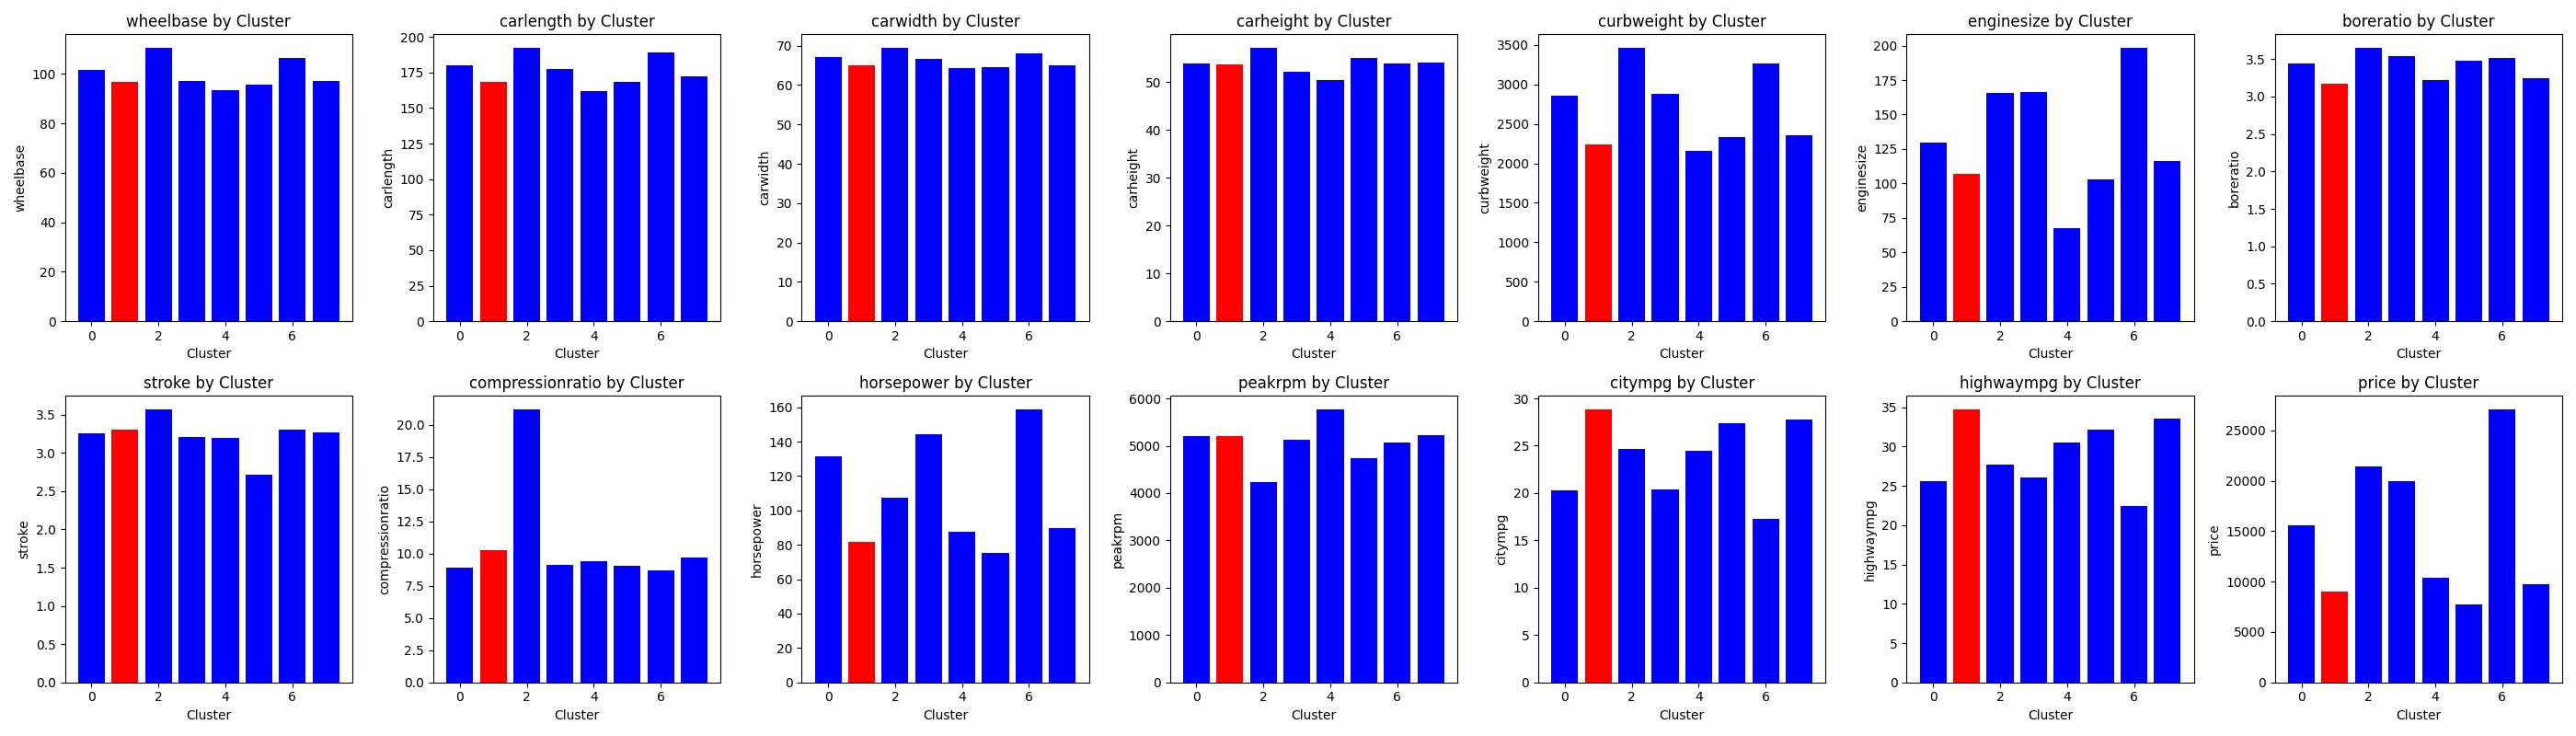
\includegraphics[width=\linewidth]{./figures/kmeans_analysis1.png}
        \caption{Bar chart analysis using kmeans clustering.}
        \label{fig:kmeans_analysis1}
    \end{subfigure}
    \hfill
    % 第二张图
    \begin{subfigure}[b]{\linewidth}
        \centering
        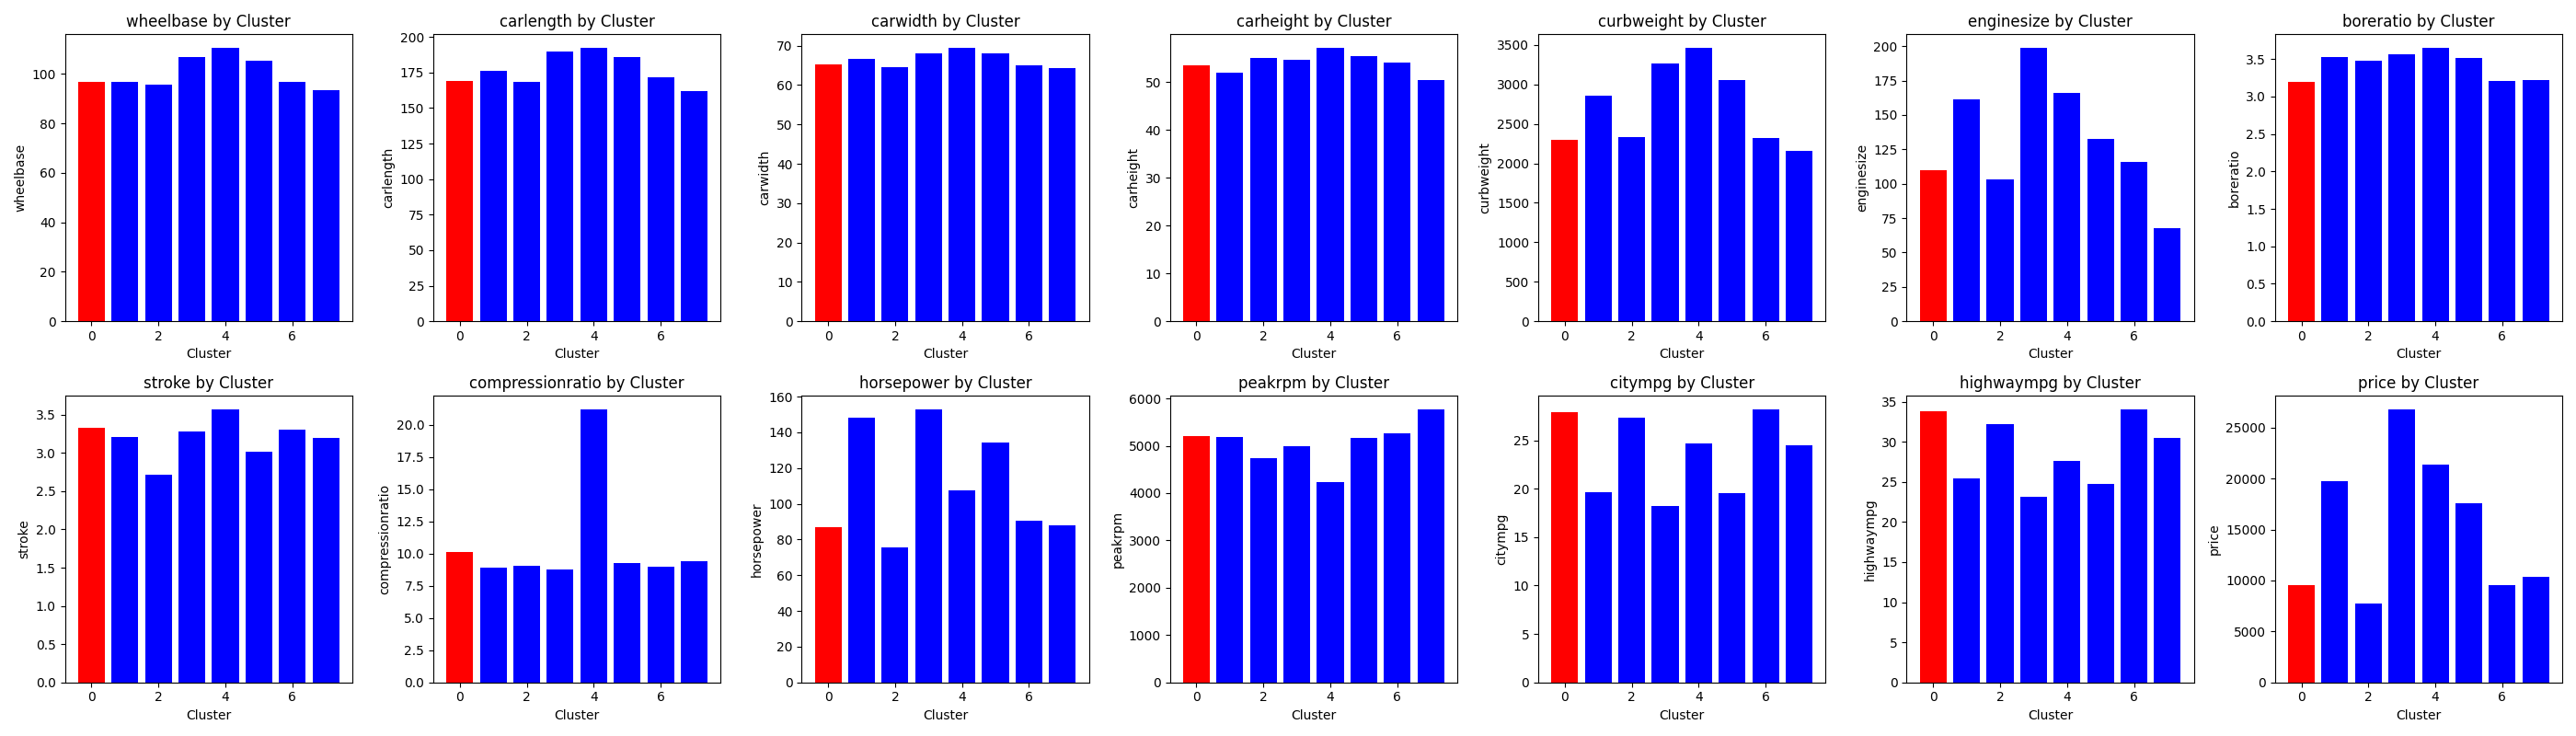
\includegraphics[width=\linewidth]{./figures/hc_analysis1.png}
        \caption{Bar chart analysis using hierarchical clustering.}
        \label{fig:hc_analysis1}
    \end{subfigure}
    % \vspace{1em} % 空隙
    % 第三张图
    \begin{subfigure}[b]{\linewidth}
        \centering
        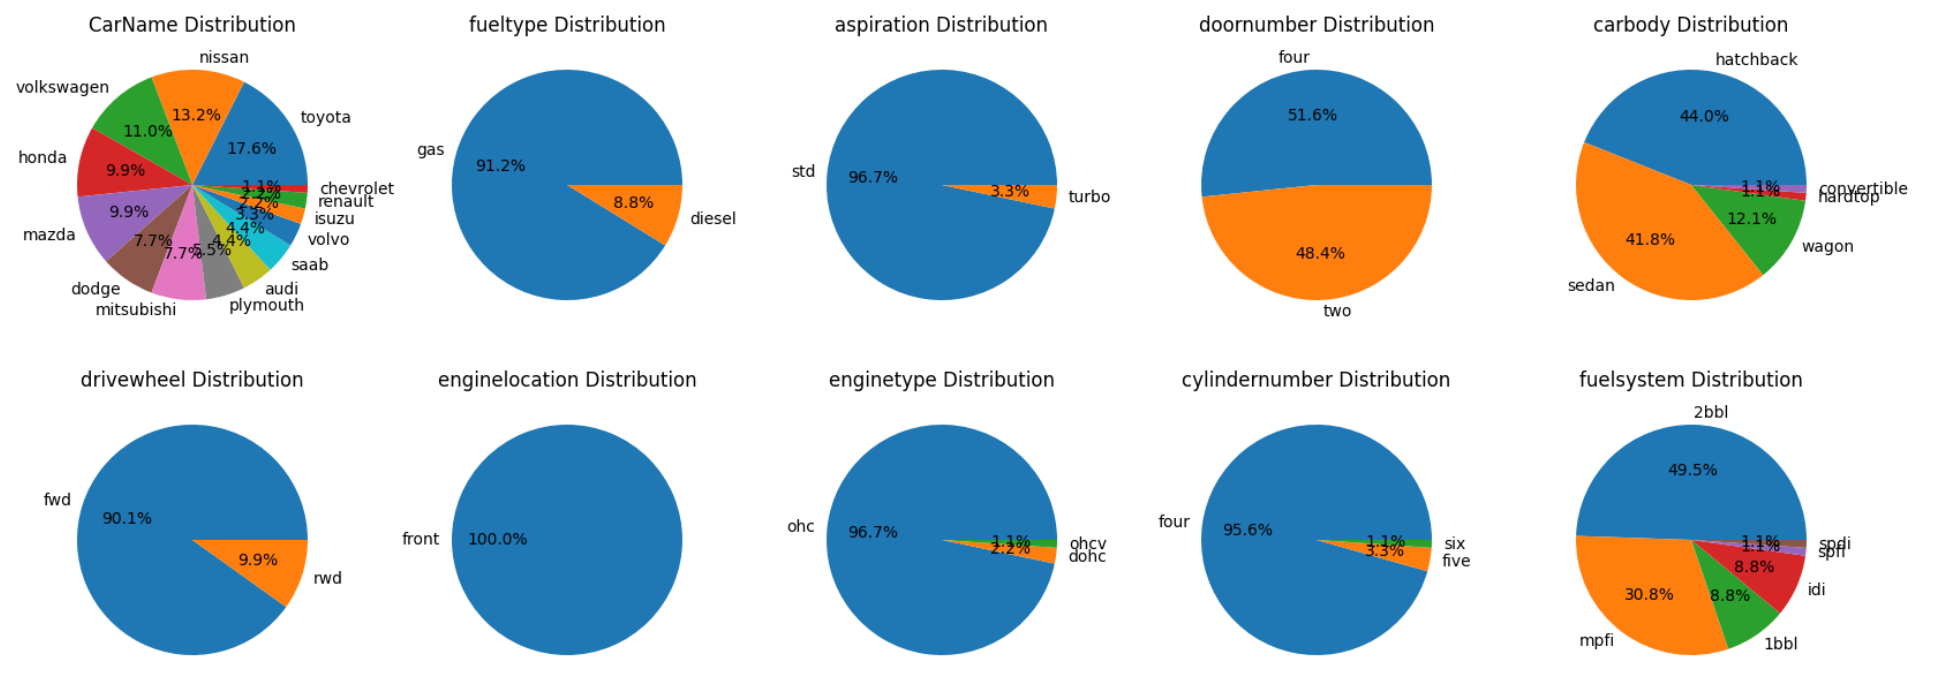
\includegraphics[width=\linewidth]{./figures/kmeans_analysis2.png}
        \caption{Pie chart analysis using kmeans clustering.}
        \label{fig:kmeans_analysis2}
    \end{subfigure}
    \hfill
    % 第四张图
    \begin{subfigure}[b]{\linewidth}
        \centering
        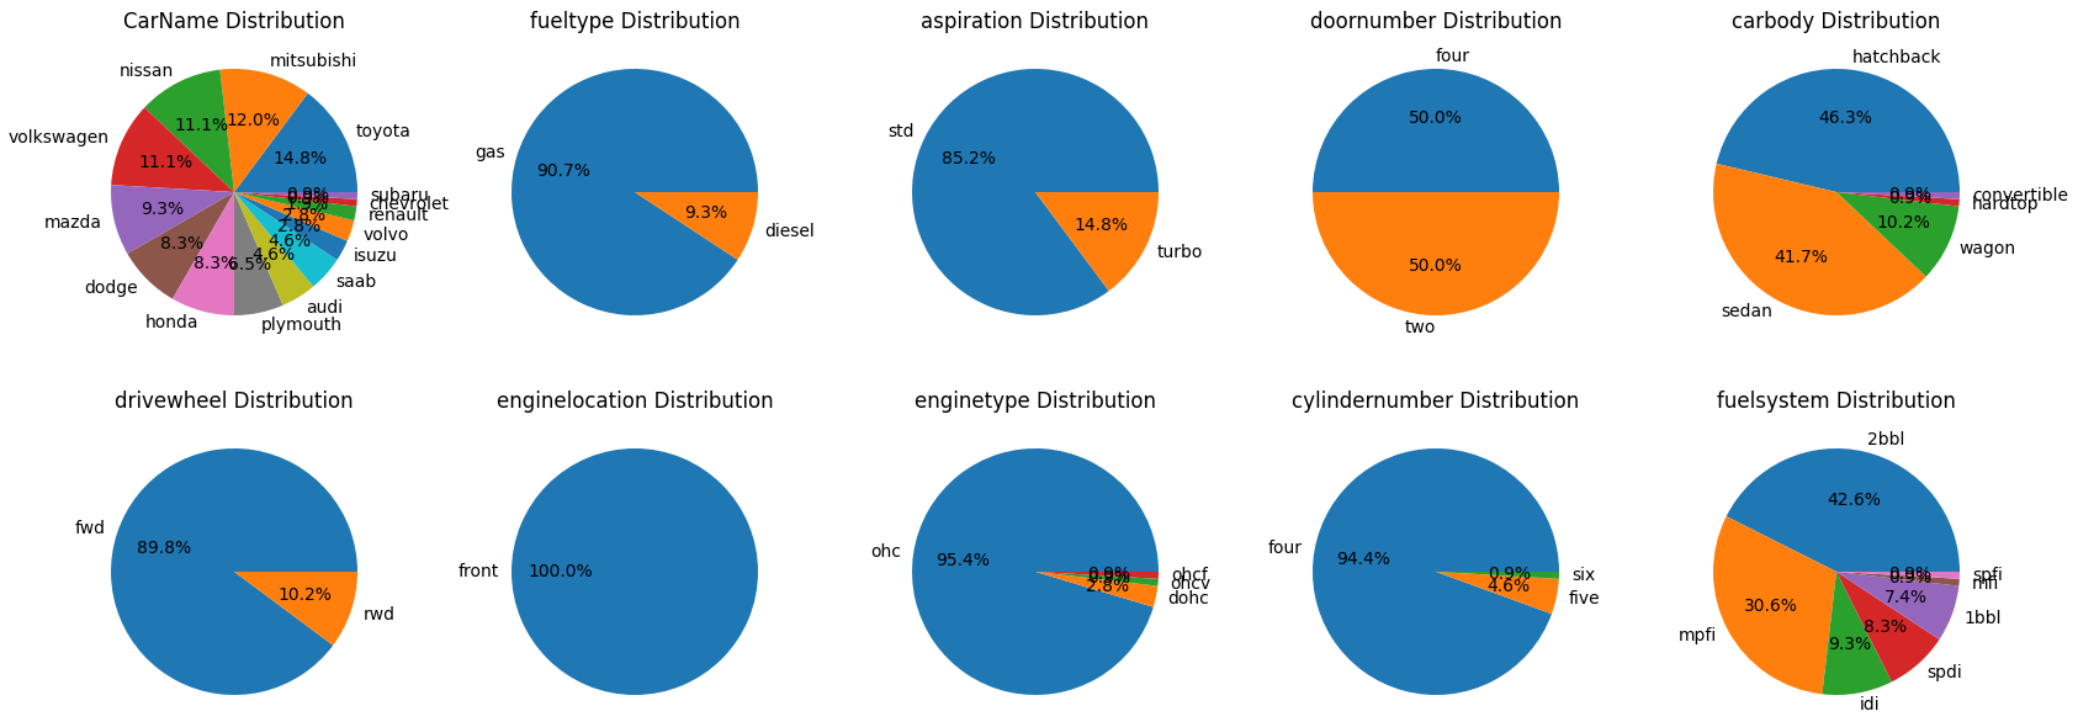
\includegraphics[width=\linewidth]{./figures/hc_analysis2.png}
        \caption{Pie chart analysis using hierarchical clustering.}
        \label{fig:hc_analysis2}
    \end{subfigure}
    \caption{}
    \label{fig:combined_analysis}
\end{figure}


\end{document}
